%!TEX root = ../thesis.tex
%*******************************************************************************
%*********************************** Signal region optimisation *********
%*******************************************************************************


\chapter{Signal region optimisation}\label{ch:signal_region_optimisation}

\graphicspath{{chapter-optimisation/Figs/Vector/}{chapter-optimisation/Figs/}}

\glsreset{sr}

In order to discover the rare \gls{susy} signals considered in the following, dedicated kinematic regions enriched in signal events, so-called \glspl{sr}, are constructed.
They are optimised such as to be sensitive to a maximum number of signal models considered in this analysis.
In this chapter, the optimisation procedures leading to the final signal regions are introduced and discussed. 

\section{Optimisation methods}

All optimisation methods used in the following require a figure of merit that is maximised in order to find configurations yielding optimal performance.
While the multidimensional cut scan and the \textit{N}--1 plots approach, introduced in \cref{sec:n-dim-scan,sec:n-1-scan}, respectively, use the binomial discovery significance $Z_\mathrm{B}$, the fit scan procedure, discussed in \cref{sec:fit-scan}, aims to maximise the area of the expected exclusion contour.

\subsection{Multidimensional cut scan}\label{sec:n-dim-scan}

 \begin{figure}
	\centering
	\begin{subfigure}[b]{0.5\linewidth}
		\centering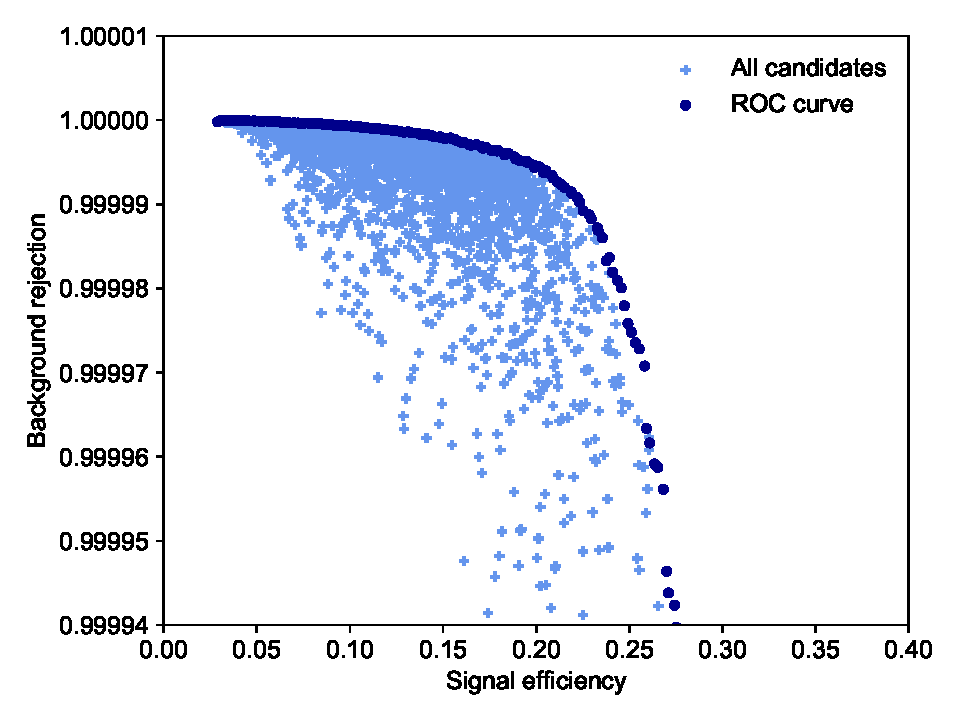
\includegraphics[width=1.0\textwidth]{N-1_cut_scan/roc_curve_thesis_plots}
		\caption{\label{fig:roc_curve}}
	\end{subfigure}\hfill
	\begin{subfigure}[b]{0.5\linewidth}
		\centering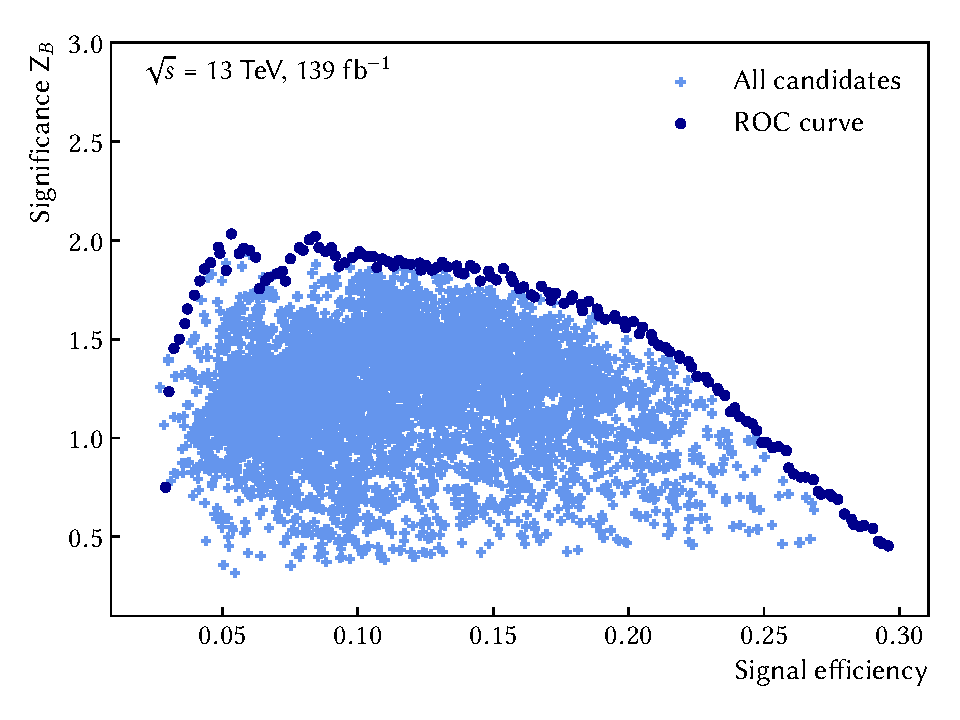
\includegraphics[width=1.0\textwidth]{N-1_cut_scan/z_vs_effs_thesis_plots}
		\caption{\label{fig:z_vs_eff}}
	\end{subfigure}\hfill

	\caption{Small $N$-dimensional cut scan using $10^4$ unique cut combinations, illustrating the approach of~\subref{fig:roc_curve} generating a \gls{roc} curve from the scanned cut combinations in order to \subref{fig:z_vs_eff} reduce the number of candidates used in computationally expensive significance calculations. The cut combination candidates forming the \gls{roc} curve (dark blue) also maximise the discovery significance. In \subref{fig:z_vs_eff}, the significance $Z_\mathrm{B}$ includes the \gls{mc} statistical uncertainty on the expected background rate and a constant 30\% systematic uncertainty.} 
	\label{fig:ahoi_examples}
\end{figure}

The first optimisation method used for designing the \glspl{sr} is an $N$-dimensional cut\footnote{In the following, the term \textit{cut} refers to a simple upper or lower requirement on kinematic observables like \eg requiring $\mt>\SI{100}{\GeV}$.} scan using $M$ observables.
For each unique combination of requirements on the set of observables considered, the expected signal and background rate as well as the statistical uncertainty on the background rate is determined from the \gls{mc} simulated events.
As this takes a considerable computational effort, it is crucial to restrict the amount of cut combinations to be tested. By comparing with distributions at preselection level, as for example those shown in \cref{fig:norm_obs}, a set of discrete cuts can be defined for each observable.
In practice, a total number of \mbox{$\mathcal{O}(10^7$--$10^8)$} cut combinations can still be tested on a single machine with a reasonable turnaround time. 

After determining the expected event rates and statistical uncertainties, the different cut combinations are binned into a predefined number of signal efficiency bins.
For each bin, the background rejection is subsequently maximised, \ie the cut combination with the highest background rejection is chosen as a candidate combination for the respective signal efficiency bin.
The assumption is that, for a fixed signal efficiency, the cut combination candidate maximising the background rejection also maximises the discovery significance $Z_\mathrm{B}$.
With the significance definition used herein, this is in general a valid assumption, as the significance tends to monotonically increase with decreasing background rate, even while the statistical uncertainty on the background estimation increases due to tighter requirements and less available \gls{mc} statistics (cf. \cref{fig:ahoi_examples}).
This procedure effectively generates a \gls{roc} curve, that can be used to perform more computationally intensive calculations, as \eg calculating different variations of the discovery significance.
The approach is illustrated in a small scan using $10^4$ cut combinations in \cref{fig:ahoi_examples}.
The cut combination candidates maximising the background rejection and thus lying on the \gls{roc} curve in \cref{fig:roc_curve} are the same candidates that maximise the discovery significance in \cref{fig:z_vs_eff}.

A common problem of $N$-dimensional scans is the concept of \textit{over-tightening} the selections given the available \gls{mc} statistics.
Since the cross sections of the \gls{susy} processes considered are many orders of magnitude smaller than those of the dominant \gls{sm} processes, it is often necessary to apply tight requirements on the kinematic observables in order to achieve a significant signal-to-background separation.
However, due to the finite amount of \gls{mc} statistics available, many of the more extreme cut combinations select kinematic regions where not enough \gls{mc} statistics are available for a reasonable estimation of the background rates.
Thus, by maximising the background rejection, it may occur that cut combinations are selected where the mere lack of \gls{mc} statistics, needed to properly estimate the background rates, causes a high significance value.
As the significance values obtained for such configurations are obviously not trustworthy, they need to be avoided. 

In the $N$-dimensional cut scan implementation used herein, the available \gls{mc} datasets are split in two statistically independent, equally sized subsets. Although resulting in an additional dilution of the available \gls{mc} statistics, this approach allows to generate two independent \gls{roc} curves and  to compute two independent values for the discovery significance for each cut combination candidate. A large difference in either the \gls{roc} curves or the significance values is an indication for statistical fluctuations as a result of over-tightened cuts. In addition, requirements on the minimum number of unweighted \gls{mc} events for different background processes, as well as the maximum allowed statistical uncertainty on a given process, can be applied. In combination, these precautions offer a good handle against statistical fluctuations. In the following, the $N$-dimensional cut scan implementation provided by \texttt{ahoi}~\cite{ahoi} is used.

\subsection[\textit{N}--1 plots]{$\makemebold{N}$--1 plots}\label{sec:n-1-scan}

Instead of performing a brute-force scan of a large set of cut combinations, a more manual approach, using iterative one-dimensional scans can be employed. In so-called `\textit{N}--1 plots', the kinematic distributions of the background components as well as representative signal processes are plotted in conjunction with the significance achieved by applying a cut on each value on the \textit{x}-axis of the one-dimensional distribution plotted. All other selection requirements, except the one on the observable plotted, are applied. This method allows to investigate the impact of a single kinematic requirement on the overall significance value. By repeatedly executing this process for each observable considered, it is possible to iteratively approach a cut combination yielding results comparable to that of a brute-force cut scan. Especially when considering a sizeable set of observables, this manual approach, however, quickly becomes very cumbersome and inefficient, and risks missing optimal cut combinations that would have been found by a brute-force approach.

For this reason, the following optimisation uses an $N$-dimensional cut scan to cover the full space spanned by the observables and scan ranges considered, while \textit{N}--1 plots are used to verify and fine-tune results obtained by the brute-force approach.

\subsection{Scans using asymptotic formulae}\label{sec:fit-scan}

The last of the optimisation methods, used in the following, relies on scans over sets of simplified profile likelihood fit configurations in order to run a simplified version of the full statistical inference machinery on a large number of signal region candidates.
While the preceding optimisation methods rely on the binomial significance computed in independent \textit{cut-and-count} signal regions, the simplified fit scans statistically combine disjunct signal regions by building a single likelihood, and compute the \textit{p}-values using the asymptotic formulae introduced in~\cref{ch:statistics}.
In addition, the simplified fits use all available signal points instead of relying on a limited set of benchmark points, and can thus derive an estimate of the expected exclusion contour for a large number of signal region candidates.
The estimation of the background event rates in the signal regions is taken from \gls{mc} simulation only and considers a constant systematic uncertainty of 30\% on the estimated event rate, correlated over all signal region bins. Statistical uncertainties on the background estimate from limited \gls{mc} statistics are also taken into account. 

As building the likelihood and executing the statistical inference takes a considerable computational effort, this method benefits from the previous optimisation steps defining promising signal region candidates worth scanning over.
In order to keep the number of configurations to be tested at a manageable level, the signal region candidates obtained from the previous methods are only varied to a limited degree, assuming that they were already close to optimal to begin with.

\section[Optimisation for the $1\ell$ search]{Optimisation for the $\makemebold{1\ell}$ search}
%\section[Optimisation for the $\boldsymbol{1\ell}$ search]{Optimisation for the $\boldsymbol{1\ell}$ search}

\begin{table}
	\centering
	\small
	\setlength\heavyrulewidth{0.2ex}
	\caption{List of observables and cut ranges used in the $N$-dimensional cut scan. All cuts are optional and allowed not to be applied at all.}
	\begin{tabular} {l c l}
		\toprule
		Observable &  & Cut values \\ 
		\midrule
		$\etmiss$ [GeV]& $>$ & $\in \{200,220,240,260,280,300,320,340\}$ \\
		$\etmiss$ significance $\mathcal{S}$ & $>$ & $\in \{5,10,15\}$ \\
		$\mt$ [GeV]& $>$ & $\in \{100, 120, 140,160,180,200,220,240,260,280, 300\}$ \\
		$\mct$ [GeV]& $>$ & $\in \{100, 120, 140,160,180,200,220,240,260,280, 300\}$ \\
		$\mbb$ lower [GeV]& $>$ & $\in \{85,90,95,100,105,110,115\}$ \\
		$\mbb$ upper [GeV]& $<$ & $\in \{130,135,140,145,150\}$ \\
		$p_\textrm{T}^\ell$ $[\SI{}{\GeV}]$& $>$ & $\in \{20, 40, 60, 80\}$ \\
		$p_\textrm{T}^\mathrm{jet1}$ [GeV]& $>$ & $\in \{50, 100, 150\}$ \\
		$p_\textrm{T}^\mathrm{jet2}$ [GeV]& $>$ & $\in \{50, 75, 100\}$ \\	
		$\upDelta R_{jj}$ & $<$ & $\in \{0.8,1.0,1.2,2.0\}$ \\
		$\upDelta R_{b\hspace{-0.06em}\bar{b}}$ & $<$ & $\in \{0.8,1.0,1.2,2.0\}$ \\
		$N_\mathrm{jet}$ & $\leq$ & $\in \{2,3,4\}$ \\			
		$\upDelta\phi (\vetmiss,\vptlep )$ [rad]& $>$ & $\in \{0.5,1.0,2.0,2.5\}$ \\
		\bottomrule					
	\end{tabular}\vspace{2mm}
	\label{tab:cut_scan}   
\end{table}

The optimisation of the signal regions for the \onelepton search benefits from the experience of past analyses investigating the same simplified model in the same final state~\cite{SUSY-2013-23,SUSY-2017-01}, but explores new observables and considers signal region configurations optimised for the integrated luminosity of the full Run~2 dataset. 

\subsection{Starting from benchmark signal points}

A total of six so-called \textit{benchmark} signal points, each representative of a different part of the model parameter space, are chosen for the first step of the optimisation procedure involving $N$-dimensional cut scans and \textit{N}--1 plots.
Apart from the variables introduced in~\cref{sec:variables}, a set of additional, potentially discriminative observables are considered in the $N$-dimensional cut scan\footnote{These variables will turn out not to be used for the final signal regions and are only introduced here for completeness of the optimisation procedure description. Representative kinematic distributions for all observables are shown as a reference in \cref{fig:additional_presel_plots}.}:
\begin{itemize}
	\item The transverse momenta of the two leading jets as well as of the lepton ($p_\textrm{T}^\mathrm{jet1}$, $p_\textrm{T}^\mathrm{jet2}$, $\ptl$). Especially for signal models with high mass differences between the electroweakinos, the transverse momenta of the lepton and the jets tend to have higher values than in \gls{sm} background processes.
	\item The object-based $\etmiss$ significance $\mathcal{S}$~\cite{met_significance:2294922}, an observable designed to quantify how genuine the reconstructed $\etmiss$ in an event is. It is determined through a hypothesis test using a log-likelihood ratio that takes into account the resolution of all objects entering the computation of $\etmiss$. As such, $\mathcal{S}$ offers good discrimination against events with a sizeable fraction of fake $\etmiss$ in the event originating, \eg, from jet mismeasurements or the non-hermeticity of the detector. Events with a large share of fake $\etmiss$ accumulate at low values of $\mathcal{S}$, while events with mostly real $\etmiss$ tend to have large values of $\mathcal{S}$. 
	\item The distance between the two leading jets $\upDelta R_{jj}$ as well as between the two \textit{b}-jets $\upDelta R_{b\hspace{-0.06em}\bar{b}}$. Especially in events with a large mass difference between the electroweakinos, the Higgs can receive a significant boost, such that the two \textit{b}-jets from the Higgs decay tend to be close together in the laboratory frame (and are also the highest-$\pt$ jets in an event), resulting in small values of both $\upDelta R_{jj}$ and $\upDelta R_{b\hspace{-0.06em}\bar{b}}$. In \gls{sm} background processes, however, the two leading (\textit{b}-)jets often do not originate from the same object and thus tend to be further apart.
	\item The azimuthal distance between the lepton $\pt$ and the missing transverse momentum, denoted by $\upDelta \phi (\makemebold{p}_\mathrm{T}^\ell, \makemebold{p}_\mathrm{T}^\mathrm{miss})$. This observable exploits the fact that the lepton and the $\etmiss$ tend to have a more back-to-back configuration in signal events than in many \gls{sm} processes where the lepton and the neutrino (the latter often responsible for a large part of the $\etmiss$ in an event) often originate from the same $W$ boson decay.
\end{itemize}

\begin{figure}
	\centering
	\begin{subfigure}[b]{0.5\linewidth}
		\centering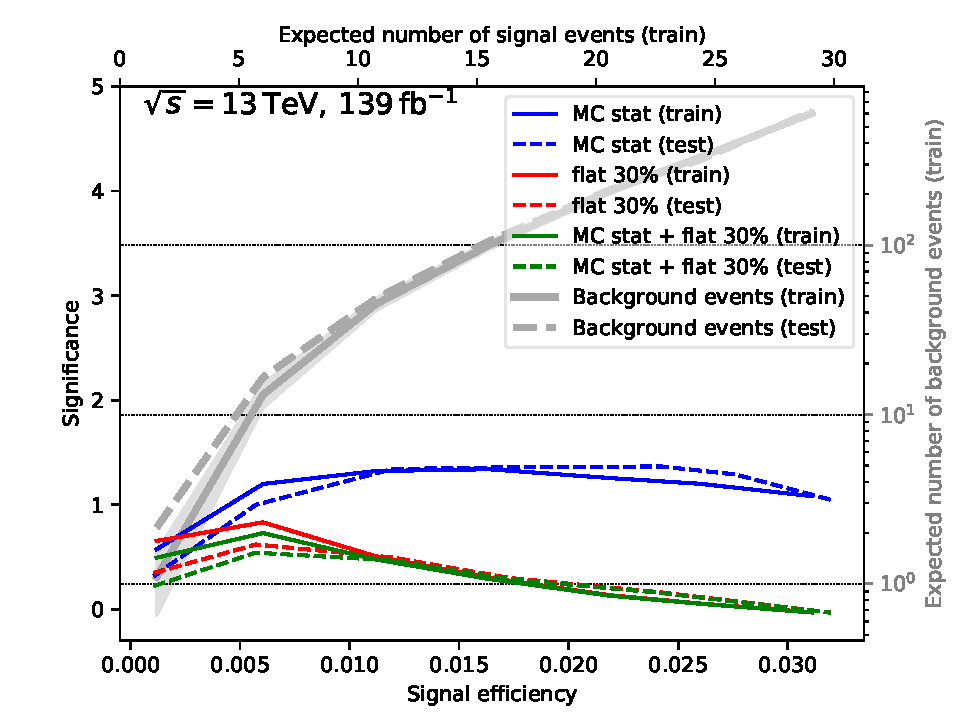
\includegraphics[width=1.0\textwidth]{N-1_cut_scan/z_vs_effs_300_150.pdf}
		\caption{$m(\charg$/$\neutr), m(\lsp) =  300, \SI{150}{\GeV}$}
	\end{subfigure}\hfill
	\begin{subfigure}[b]{0.5\linewidth}
		\centering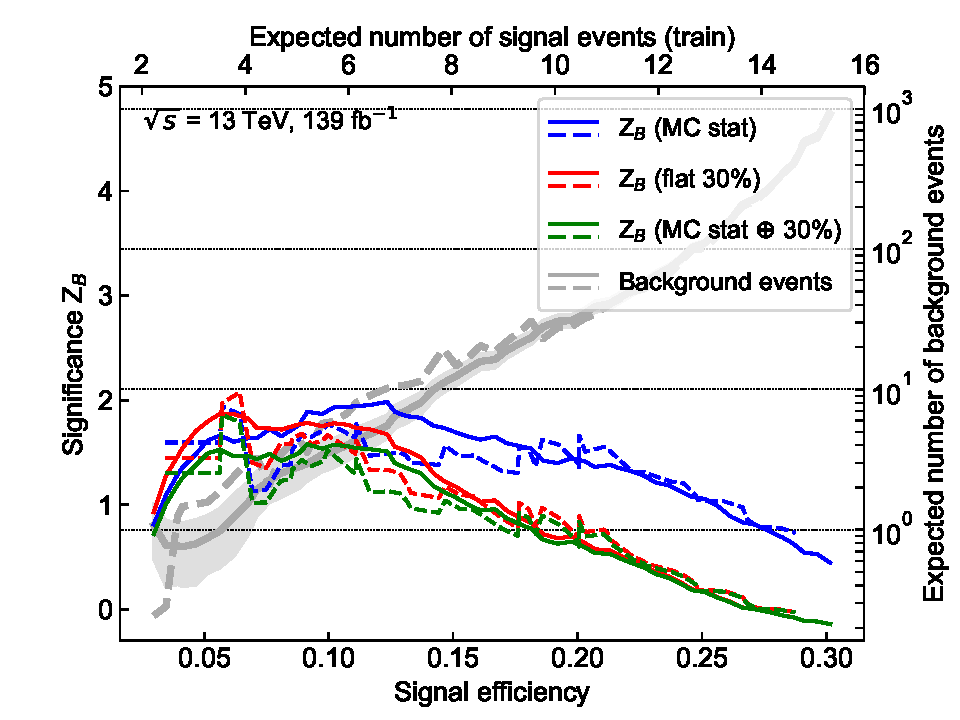
\includegraphics[width=1.0\textwidth]{N-1_cut_scan/z_vs_effs_800_250.pdf}
		\caption{$m(\charg$/$\neutr), m(\lsp) =  800, \SI{250}{\GeV}$}
	\end{subfigure}\hfill

	\caption[N-dimensional cut scan results]{Results of the $N$-dimensional cut scan for two representative benchmark points. The binomial discovery significance $Z_\mathrm{B}$ is plotted against the signal efficiency for different uncertainty configurations. Additionally, the expected \gls{sm} background event rates are shown (grey), including their statistical uncertainties for one of the two statistically independent samples (grey shaded area). The solid and dashed lines represent the two statistically independent subsets that the \gls{mc} samples are split into.}
	\label{fig:results_z_vs_eff}
\end{figure}

In order to avoid selecting cut combination candidates with over-tightened selection criteria compared to the available \gls{mc} statistics, constraints are applied on the relative statistical uncertainty on the background, and on the number of unweighted \gls{mc} events passing the cut combination candidates.
Cut combinations are only considered if they result in less than 50\% relative statistical uncertainty on the total background.
In addition, all cut combinations need to result in at least five unweighted \gls{mc} events for each of the three major backgrounds, $\ttbar$, single top and $\wjets$.

The discrete selection possibilities for each of the observables are shown in \cref{tab:cut_scan}.
A preselection of a lepton and exactly two \textit{b}-jets (and thus at least two jets overall in the event) is always applied. Requirements on the different observables in~\cref{tab:cut_scan} are optional and do not need to be applied by the optimisation algorithm.
The results of the brute-force $N$-dimensional cut scans for each benchmark signal point can be visualised by plotting the expected discovery significance $Z_\mathrm{B}$ against the signal efficiency.
\Cref{fig:results_z_vs_eff} shows the results of two such cut scans using two of the benchmark signal points.
The corresponding plots for the remaining benchmark points are shown in~\cref{fig:results_z_vs_eff_rest}. In these figures, the binomial significance is calculated for different uncertainty configurations for each of the two statistically independent subsets.
In addition, the expected background rate is shown for each subset.
A cut combination with high achieved significance can be chosen, while avoiding statistical fluctuations and over-tightening.
The cut combinations chosen for each benchmark point, after a round of \textit{N}--1 plots, are shown in~\cref{tab:cut_scan_results}. The \textit{N}--1 plots, shown in~\cref{fig:results_n1_800_0,fig:results_n1_800_150,fig:results_n1_800_250,fig:results_n1_600_300,fig:results_n1_400_200,fig:results_n1_300_150}, are used to validate and fine-tune the cut values obtained through the cut scan and allow to identify and remove cuts on observables that do not contribute significantly to the achieved $Z_\mathrm{B}$ value.
From the 12 observables initially considered, only six (excluding the \textit{b}-jet multiplicity technically not part of the scan) are part of the optimised cut combination candidates.
The remaining observables turned out not to significantly improve the sensitivity and are therefore dropped in the following.


\begin{table}
	\begin{center}
	\small
			\begin{tabular} {l c c c c c c c}
				\toprule
				Observable &  $(300,150)$ & $(400,200)$ & $(600,300)$  & $(800,250)$ & $(800,150)$ & $(800,0)$ \\
				\midrule
				$N_{b\mathrm{-jet}}$ &  2 & 2 & 2 & 2 & 2 & 2 \\
				$N_\mathrm{jet}$ & 2 & 2 & 2 -- 3 & 2 -- 3  & 2 -- 3 & 2 -- 3\\
				$\mbb$  $[\SI{}{\GeV}]$& $[105-135]$ & $[100-140]$ & $[100-140]$ & $[95-145]$ & $[95-145]$ & $[95-145]$ \\
				$\met$ $[\SI{}{\GeV}]$ & $>240$ & $>240$ & $>240$ & $>240$ & $>240$  & $>240$\\
				$m_\mathrm{CT}$ $[\SI{}{\GeV}]$ &  $>200$ & $>240$ & $>260$ & $>260$ & $>260$   & $>280$ \\
				$m_\mathrm{T}$ $[\SI{}{\GeV}]$ &  $>100$ & $>120$ & $>140$ & $>200$ & $>240$ & $>240$ \\
				$\mlb$ $[\SI{}{\GeV}]$ &  -- & -- & $>150$ & $>120$ & $>120$ & $>120$ \\
				\midrule
				$Z_\mathrm{B}$ $[\sigma]$ & \multicolumn{1}{c}{0.8} & \multicolumn{1}{c}{1.9} & \multicolumn{1}{c}{2.1} & \multicolumn{1}{c}{1.8} & \multicolumn{1}{c}{2.2} & \multicolumn{1}{c}{2.3} \\
				\bottomrule
			\end{tabular}
		\caption{Optimal cut combination for each benchmark signal point obtained with a brute force cut scan and a round of \textit{N}--1 plots. The parameters of the benchmark points are $m(\charg$/$\neutr)$ and $m(\lsp)$, both given in $\SI{}{\GeV}$. The significance is computed for \onethirtynineifb with the binomial discovery significance $Z_\mathrm{B}$ and includes MC statistical uncertainty as well as a constant 30\% systematic uncertainty. A dash `--' is used where no requirement on the respective observable is applied.}
		\label{tab:cut_scan_results}
	\end{center}
\end{table}




\subsection{Towards final signal regions}\label{sec:towards_signal_regions}

The optimal cut combinations obtained for the benchmark signal points, shown in~\cref{tab:cut_scan_results}, need to be consolidated into a final set of signal regions.
From~\cref{tab:cut_scan_results}, it can be concluded, that all benchmark points favour a common baseline selection including exactly two \textit{b}-jets, possibly one additional light jet, a Higgs mass window requirement of roughly $\mbb\in [100,140]$~$\SI{}{\GeV}$, and $\etmiss > \SI{240}{\GeV}$.
The remaining requirements on $\mt$, $\mct$ and $\mlb$ are, however, not easily consolidated into a single signal region, as they vastly differ depending on the model parameter space and kinematic regime represented by each benchmark point.

It can already be seen from the normalised distributions in~\cref{fig:norm_obs,fig:norm_obs_app}, that signal points from different kinematic regimes in the parameter space would in principle prefer different requirements on all three of these observables.
Designing a single signal region that achieves optimal sensitivity to the entire parameter space studied, is thus not possible.
Instead, a more generalised configuration is chosen, defining multiple signal region bins orthogonal to each other through their requirements on $\mt$ and $\mct$.
Being mutually exclusive, such signal region bins can be statistically combined in a single likelihood and can be used in a simultaneous fit to data, effectively creating a two-dimensional shape-fit in these observables.
Such a shape-fit configuration allows to exploit the differences in shape between signal and background distributions, and is able to accommodate the varying shapes of signal points from different regions in the parameter space, making it an ideal statistical tool to cover a wide range of kinematic regimes.

The optimal number of bins as well as values of the individual bin edges in both distributions depends on the available \gls{mc} statistics and is determined using the simplified fit scans introduced in~\cref{sec:fit-scan}.
The \gls{mc} statistical uncertainties, as well as a systematic uncertainty of 30\%, correlated over all bins, are considered in each configuration.
The number of bins is varied in each direction ($\mt$ and $\mct$) between two and five using different bin edges, varied within ranges determined by the optimal cut values obtained for the benchmark points.
As configurations with more bins could, in some circumstances, potentially benefit from the additional \gls{mc} statistics resulting from looser selection criteria on the remaining variables, the previously consolidated baseline selection is also allowed to vary to some extent.
Finally, although not expected to yield better performance, configurations with multiple orthogonal signal region bins in $\etmiss$ or $\mbb$ are also included in the scan.
A subset of the investigated candidates is illustrated in~\cref{fig:fit_scan_optimisation}, showing the nominal expected exclusion limit at 95\% without uncertainty bands.
Configurations with multiple, disjoint patches of excluded areas in the parameter space are discarded, as they typically result from high statistical fluctuations.

\begin{figure}
\floatbox[{\capbeside\thisfloatsetup{capbesideposition={right,center},capbesidewidth=0.35\textwidth}}]{figure}[\FBwidth]
{\caption{Expected exclusion contours obtained from a subset of the signal region candidates. The background estimate is directly taken from \gls{mc} and includes \gls{mc} statistical uncertainty as well as an uncorrelated scale uncertainty of 30\%. For the sake of visibility, only the nominal contours are shown (without uncertainty bands). Configurations resulting in multiple, disjoint patches of excluded areas are rejected.}\label{fig:fit_scan_optimisation}}
{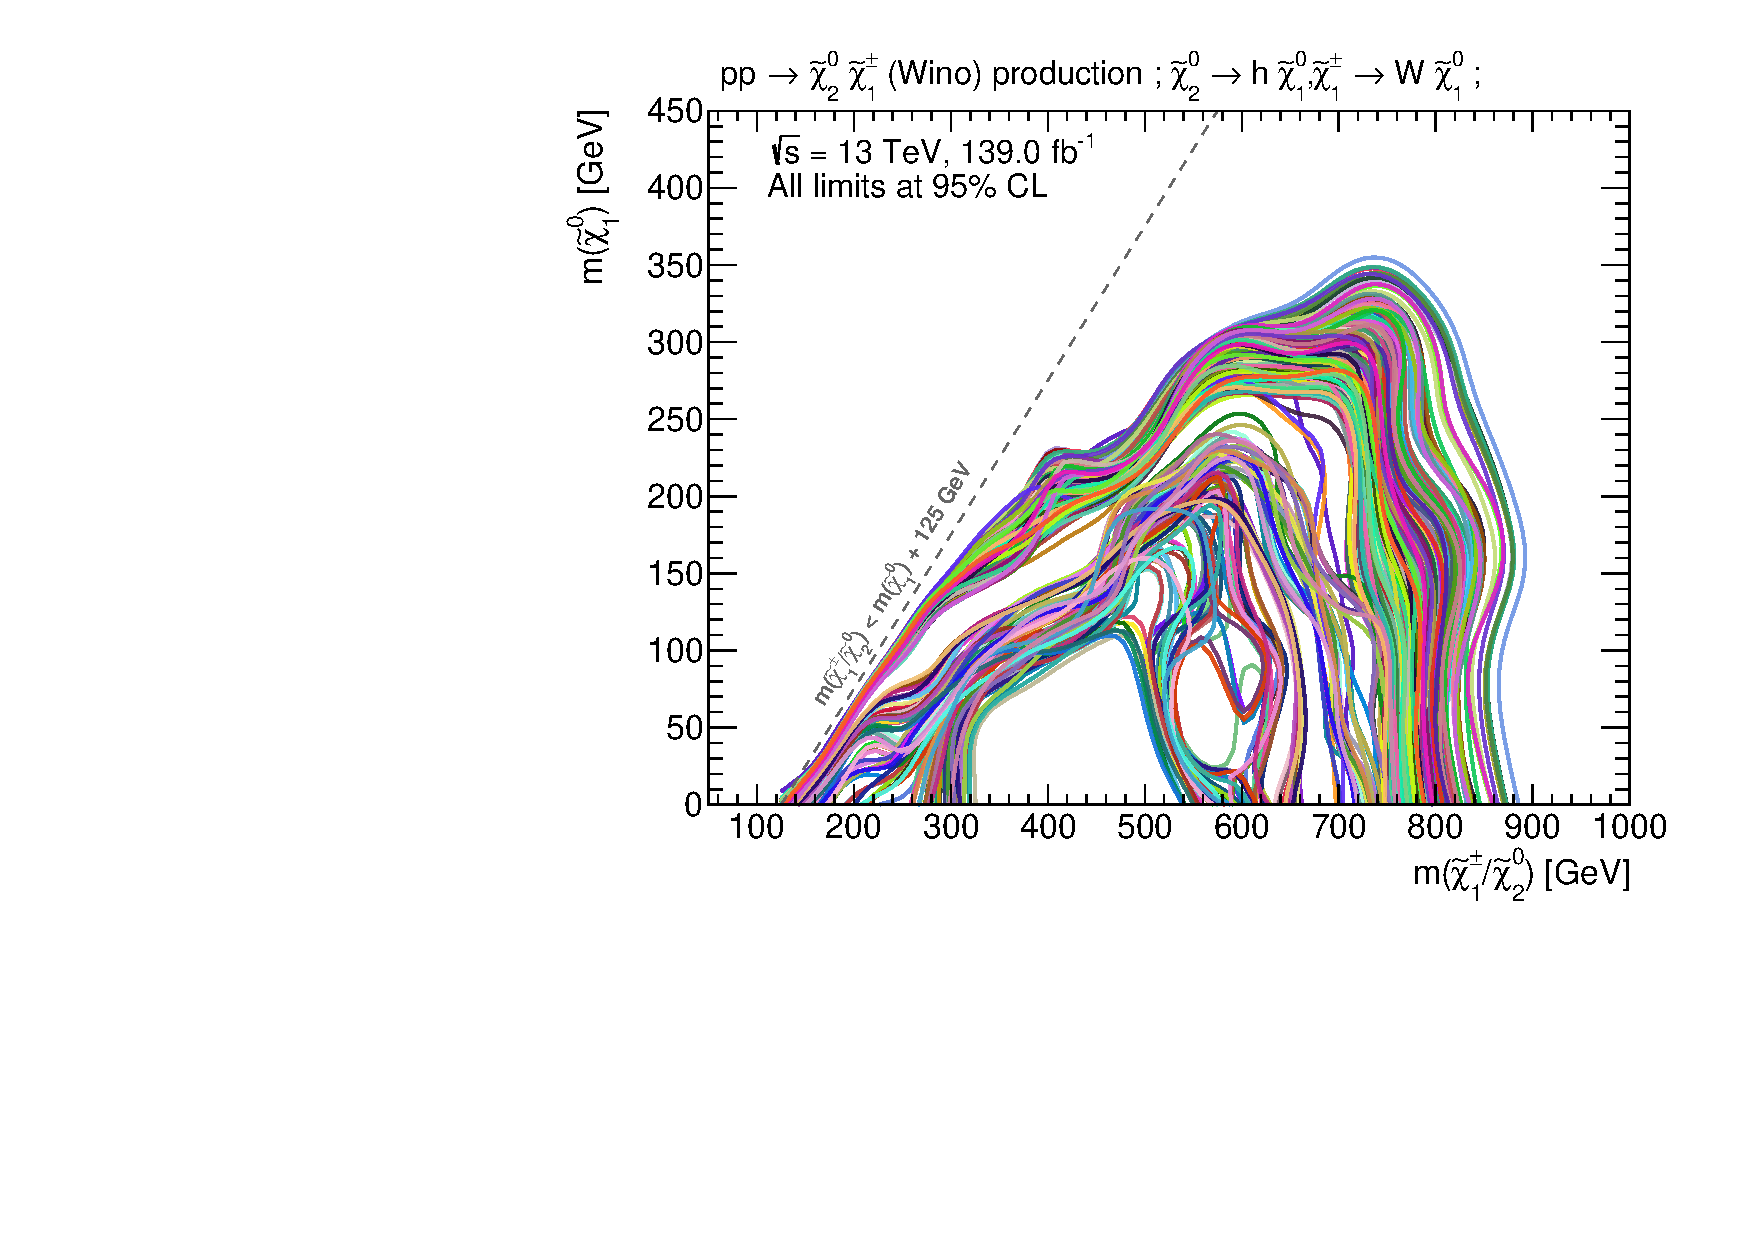
\includegraphics[width=0.60\textwidth]{HF/batch_compare}}
\end{figure}

As expected from~\cref{tab:cut_scan_results}, the best performing configurations define multiple signal region bins in the $\mt$ and $\mct$ distributions, while keeping a constant baseline selection on the remaining observables.
\Cref{fig:plot_binnings} shows a comparison of the expected exclusion contour for exemplary two-dimensional shape-fit configurations, using signal regions binned in ($\mt$, $\etmiss$), ($\mt$, $\mbb$) or ($\mt$, $\mct$).
The setup using a two-dimensional shape-fit in $\mt$ and $\mct$ clearly maximises the expected excluded area.
%In addition, this configuration also leads to optimal sensitivity within the expected limit, as is illustrated in~\cref{fig:plot_binnings_cls}.
Finally, applying a requirement on high values of $\mlb$ in the highest $\mt$ bins has been shown (cf.~\cref{fig:plot_mlb1_cls}) to further increase sensitivity to signal models with high mass differences. 

In~\cref{fig:previous_analysis_comparison}, the fully optimised two-dimensional shape-fit configuration is compared with the signal regions of the previous iteration of the search~\cite{SUSY-2017-01}, scaled up to the integrated luminosity of the full Run~2 dataset.
It can clearly be seen that a significant improvement in sensitivity is achieved through the introduction of the two-dimensional shape-fit strategy.

 \begin{figure}
	\centering
	\begin{subfigure}[b]{0.5\linewidth}
		\centering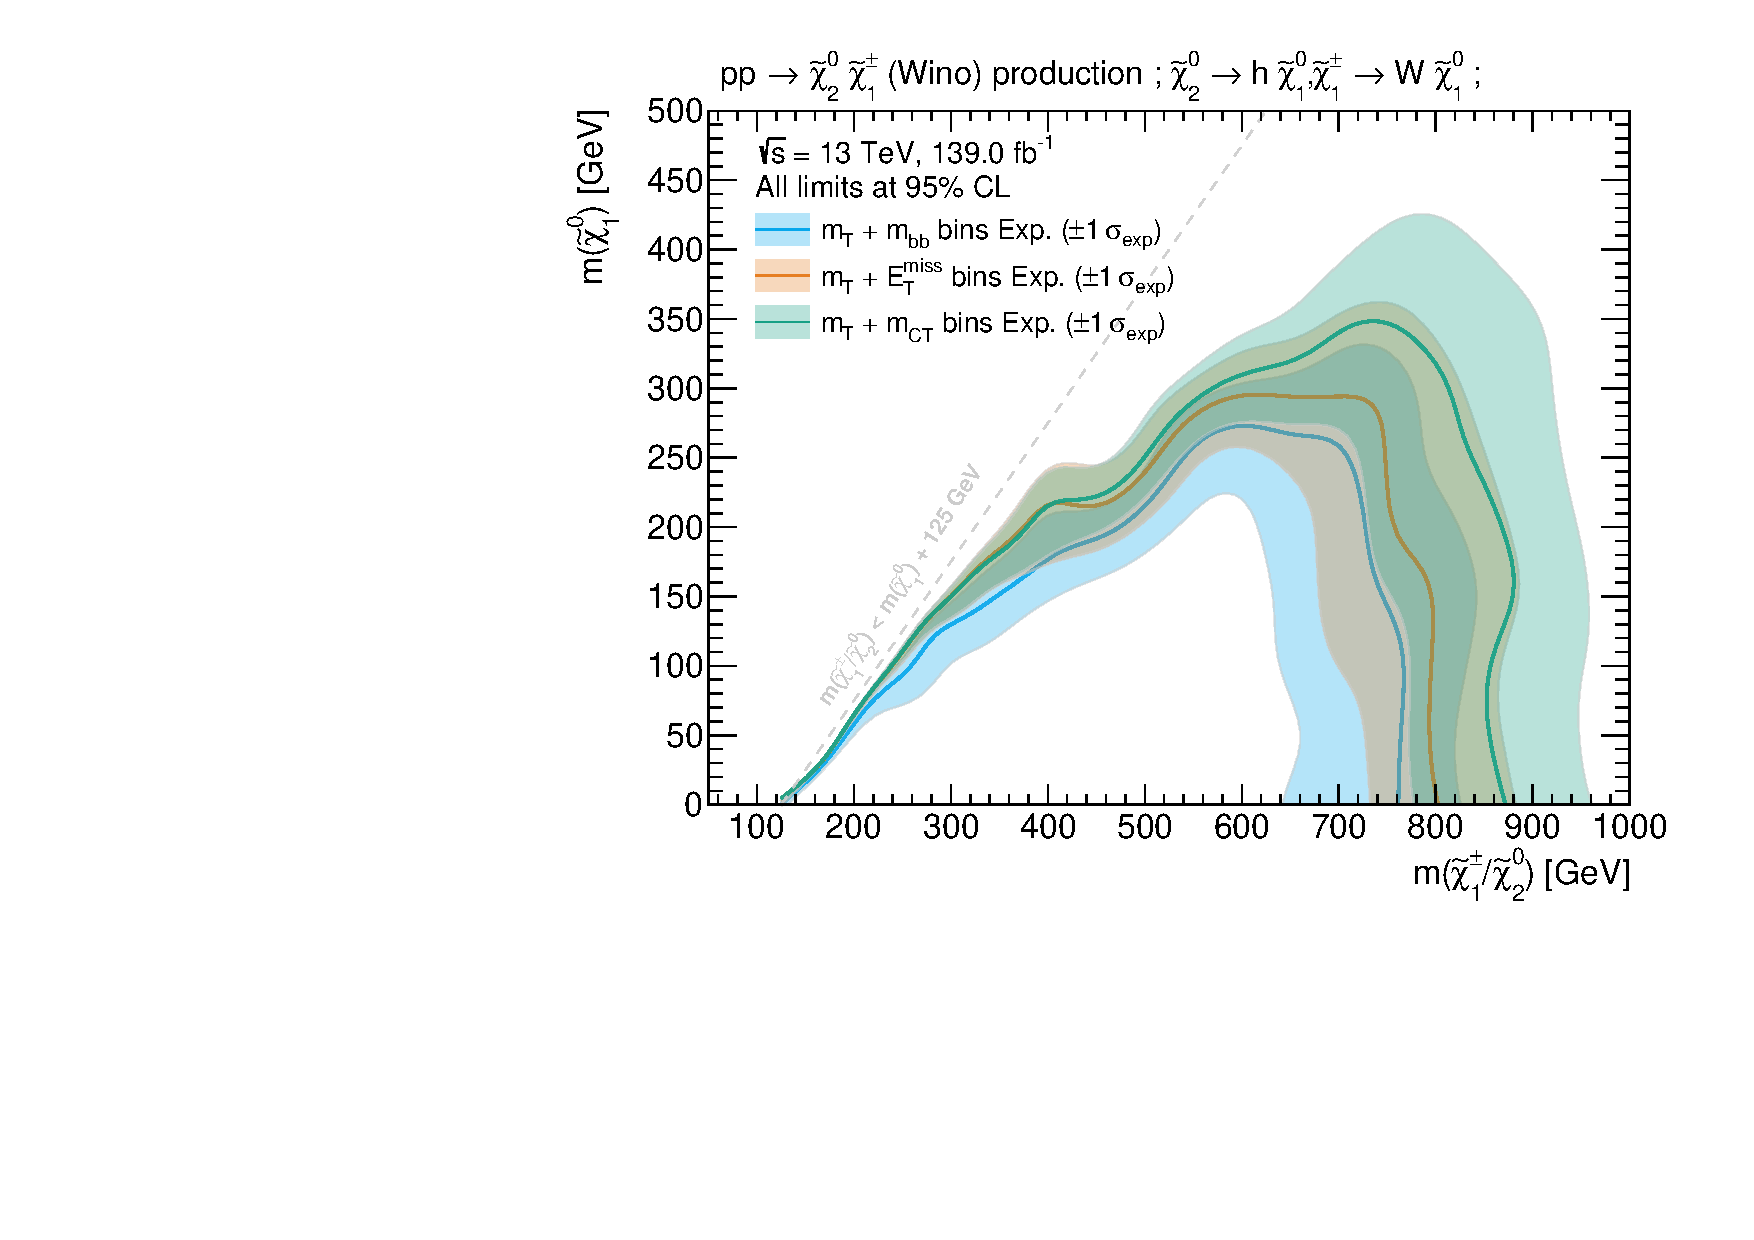
\includegraphics[width=1.0\textwidth]{HF/plot_binnings}
		\caption{\label{fig:plot_binnings}}
	\end{subfigure}\hfill
	\begin{subfigure}[b]{0.5\linewidth}
		\centering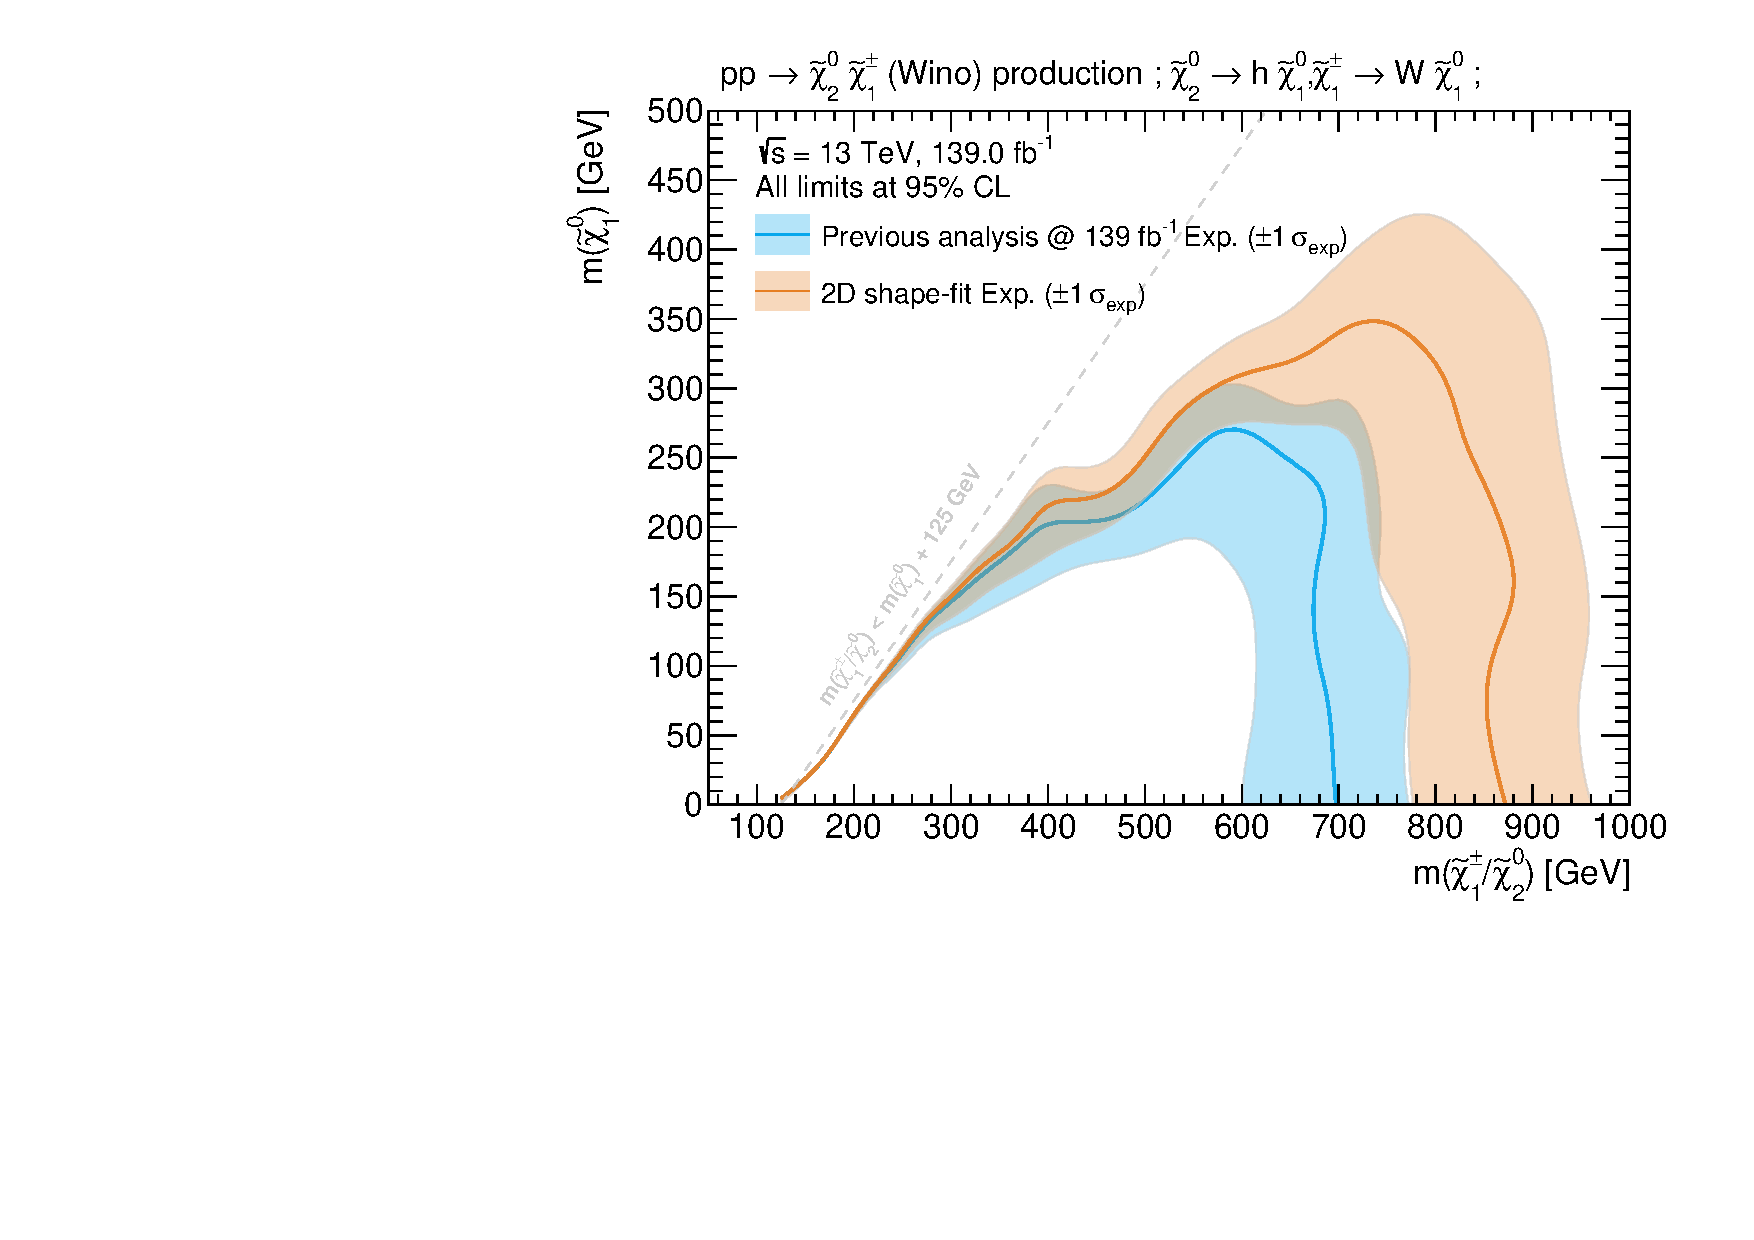
\includegraphics[width=1.0\textwidth]{HF/plot_2d_shapefit}
		\caption{\label{fig:previous_analysis_comparison}}
	\end{subfigure}\hfill

	\caption{Comparison of different shape-fit configurations. Figure~\subref{fig:plot_binnings} compares three different two-dimensional shape-fit configurations using $3\times 3$ bins in ($\mt$, $\etmiss$), ($\mt$, $\mbb$) and ($\mt$, $\mct$). Figure~\subref{fig:previous_analysis_comparison} compares the two-dimensional shape-fit in $\mt$ and $\mct$ to the signal regions of the previous analysis iteration signal regions scaled to \onethirtynineifb. All exclusion limits shown are expected limits at 95\% CL, using \gls{mc} statistical and 30\% systematic uncertainties.}
	\label{fig:results_HF_scans}
\end{figure}


\section{Signal region definitions}\label{sec:signal_region_definitions}

\begin{table}
	\begin{center}
		\begin{tabular} {l | c c c }
			\toprule
				&  \textbf{SR-LM} & \textbf{SR-MM} & \textbf{SR-HM} \\
			\midrule
			$N_{\mathrm{lepton}}$ & \multicolumn{3}{c}{$=$ 1}\\
			$\ptl$ [\GeV] & \multicolumn{3}{c}{ $>7(6)$ for $e$($\mu$)} \\
			$N_\mathrm{jet}$ & \multicolumn{3}{c}{$=$ 2 or 3}\\
			$N_{b\textrm{-jet}}$ &\multicolumn{3}{c}{$=$ 2} \\
			$\met$ $[\SI{}{\GeV}]$ & \multicolumn{3}{c}{$>240$}\\
			$\mbb$  $[\SI{}{\GeV}]$ & \multicolumn{3}{c}{$\in [100,140]$}\\
			$m(\ell,b_1)$ $[\SI{}{\GeV}]$ & -- & -- & $>120$ \\
			\midrule
			%                        \mt $[\SI{}{\GeV}]\mathrm{(excl.)}$&   $\in [100,160]$ & $\in [160,240]$ & $\in [240,\infty]$ \\
			$\mt$ $[\SI{}{\GeV}]~\mathrm{(excl.)}$&   $\in [100,160]$ & $\in [160,240]$ & $>240$ \\
			
			
			$\mct$ $[\SI{}{\GeV}]~\mathrm{(excl.)}$ &\multicolumn{3}{c}{ $ \{ \in [180,230]$,\,$\in [230,280]$, $>280  \}$}\\
			%                        &\multicolumn{3}{c}{ $\in [180,230]$}\\
			%                        \mct $[\SI{}{\GeV}]\mathrm{(excl.)}$ & \multicolumn{3}{c}{ $\in [230,280]$} \\   
			%                         & \multicolumn{3}{c}{ $>280$}\\
			%                         & \multicolumn{3}{c}{ $\in [280,\infty]$}\\
			
			\midrule
			$\mt$ $[\SI{}{\GeV}]~\mathrm{(disc.)}$&   $>100$ & $>160$ & $>240$ \\
			$\mct$ $[\SI{}{\GeV}]~\mathrm{(disc.)}$ & \multicolumn{3}{c}{ $>180$}\\
			\bottomrule
		\end{tabular}
		\caption{Overview of the selection criteria for the signal regions. Exclusion \glspl{sr} (`excl.') are defined for model-dependent limits, and discovery \glspl{sr} (`disc.') are defined for model-independent upper limits. A dash `--' is used where no requirement on the respective observable is applied.} 
		\label{tab:SignalRegionDef}
	\end{center}
\end{table}

An overview of the final signal region definitions is provided in~\cref{tab:SignalRegionDef}.
Based on the previously discussed results, three signal regions bins in $\mt$ are defined, optimised for different regimes in the \mbox{$\charg$/$\neutr$} and $\lsp$ mass difference. According to the mass difference regime targeted, they are aptly called low (SR-LM), medium (SR-MM), and high (SR-HM) mass signal regions, respectively.
While SR-LM targets the smallest values of $\mt$, SR-MM and SR-HM target progressively increasing values of $\mt$.
All three signal regions are further divided into three $\mct$ bins each, resulting in a total of nine disjoint signal region bins. The signal region with the highest requirement on $\mt$ (SR-HM) also requires $\mlb>\SI{120}{\GeV}$, for the reason explained previously.
All three signal regions otherwise share a common set of requirements on the number of jets, $\etmiss$ and $\mbb$.
As shape-fits are by construction highly model-dependent\footnote{The signal shapes need to be known in order to estimate the expected signal rates in multiple, disjoint signal region bins.}, these \glspl{sr} will be used for deriving model-dependent limits in the case where no significant excess, compared to the expected \gls{sm} background rate, is seen in data.
For this reason, the shape-fit regions will be referred to as \textit{exclusion} regions in the following. A graphical representation of the nine exclusion signal region bins is shown in~\cref{fig:sr_strategy}.
The kinematic distributions in SR-LM, SR-MM and SR-HM are shown as \textit{N}--1 plots in \cref{fig:Wh_reopt_second_round_n1_srlm,fig:Wh_reopt_second_round_n1_srmm,fig:Wh_reopt_second_round_n1_srhm}.

For evaluating a potential excess in data compared to the expected background rate, a second set of signal regions is derived from the optimised shape-fit setup.
For each of the three bins in the transverse mass (SR-LM, SR-MM, and SR-HM), the three $\mct$ bins are summed up and the upper bound on $\mt$ is removed (if present).
This results in three \textit{cut-and-count} signal regions in which only the total number of events after the selection is relevant. Since no information about the shape of the distribution of signal events is used, these so-called \textit{discovery} regions make minimal model assumptions, and can be used to constrain any \gls{bsm} physics process for which the expected event rates in one or multiple discovery signal regions are known (cf.~\cref{sec:model_independent_limits}).
In case no significant excess over the \gls{sm} expectation is seen in data, the discovery \glspl{sr} can be used to derive upper limits on the visible cross section of physics beyond the \gls{sm}, \ie the apparent cross section of \gls{bsm} processes including the acceptance and efficiency of the signal region selections. 

% -------------------------------------------------------------------------------------------------------
\FloatBarrier
\newpage
% -------------------------------------------------------------------------------------------------------

%\begin{figure}
%\floatbox[{\capbeside\thisfloatsetup{capbesideposition={right,center},capbesidewidth=0.5\textwidth}}]{figure}[\FBwidth]
%{\caption{Configuration of the exclusion signal regions. Nine signal region bins are defined on $\mt$ and $\mct$ within the Higgs mass window. All signal regions can be statistically combined using a single likelihood, effectively resulting in a two-dimensional shape-fit.}\label{fig:sr_strategy}}
%{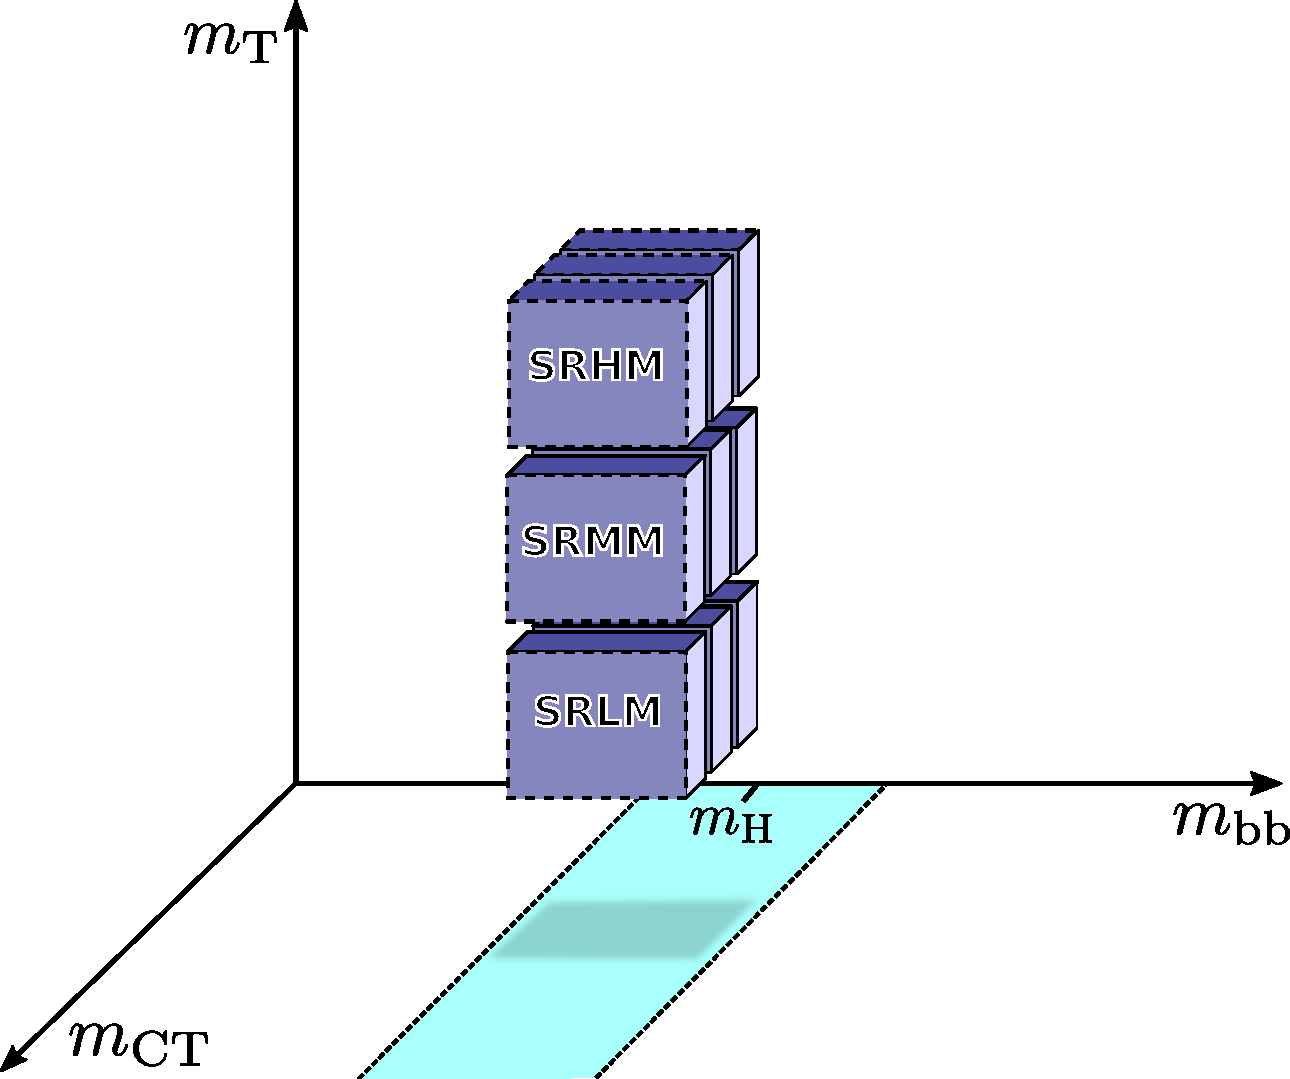
\includegraphics[width=0.45\textwidth]{strategy_2}}
%\end{figure}

\begin{figure}
	\centering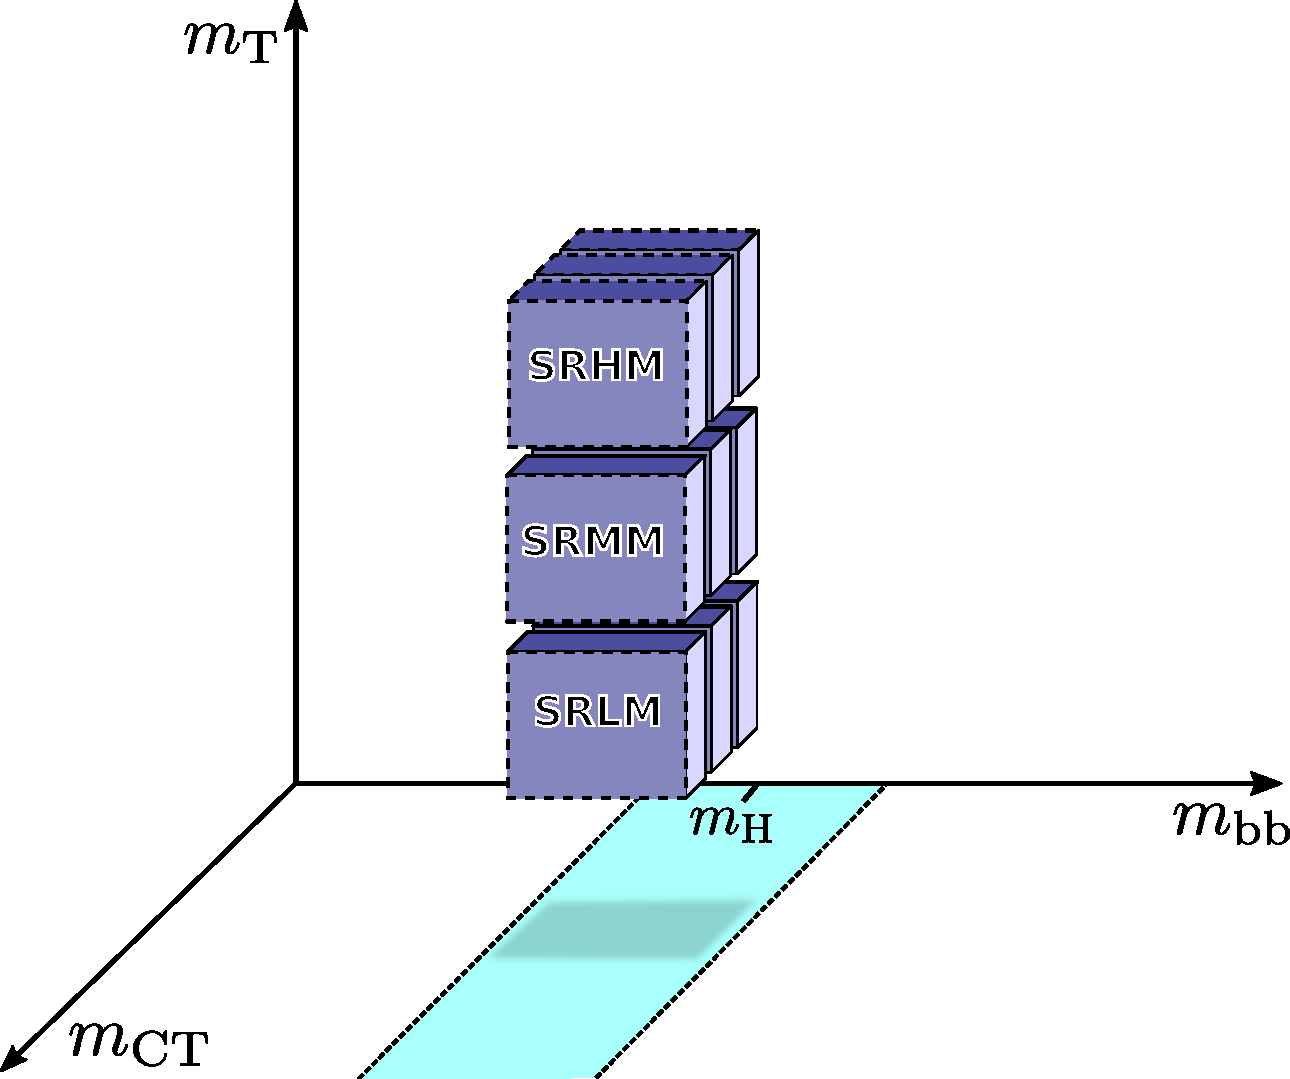
\includegraphics[width=0.6\textwidth]{strategy_2}
	\caption{Configuration of the exclusion signal regions. Nine signal region bins are defined in $\mt$ and $\mct$ within the Higgs mass window. All signal regions can be statistically combined using a single likelihood, effectively resulting in a two-dimensional shape-fit.}\label{fig:sr_strategy}
\end{figure}

\begin{figure}
	\centering
	\begin{subfigure}[b]{0.45\linewidth}
		\centering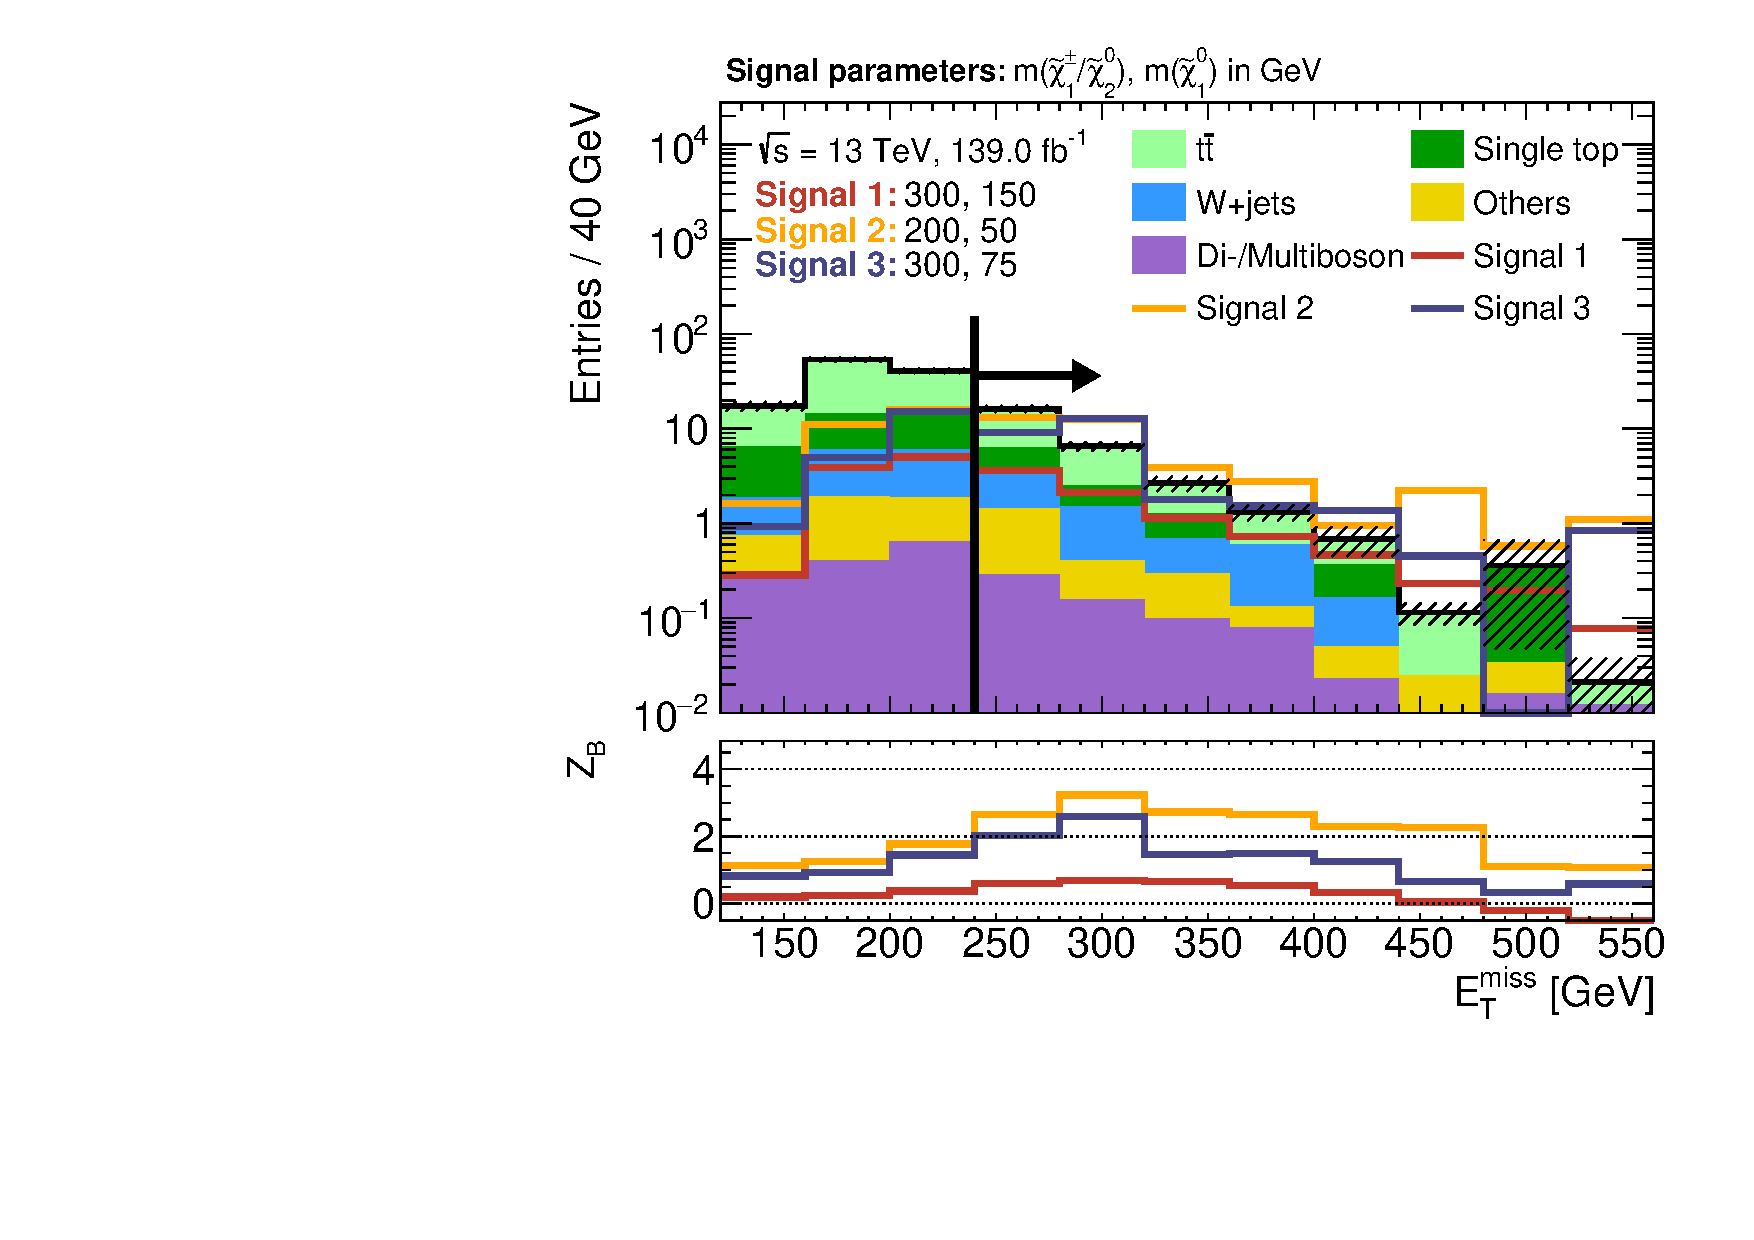
\includegraphics[width=\textwidth]{n1_SRLM_mct_bins/met.pdf}
		\vspace{-2em}
		\caption{\label{fig:Wh_reopt_second_round_n1_srlm_met}}
	\end{subfigure}%
	\begin{subfigure}[b]{0.45\linewidth}
		\centering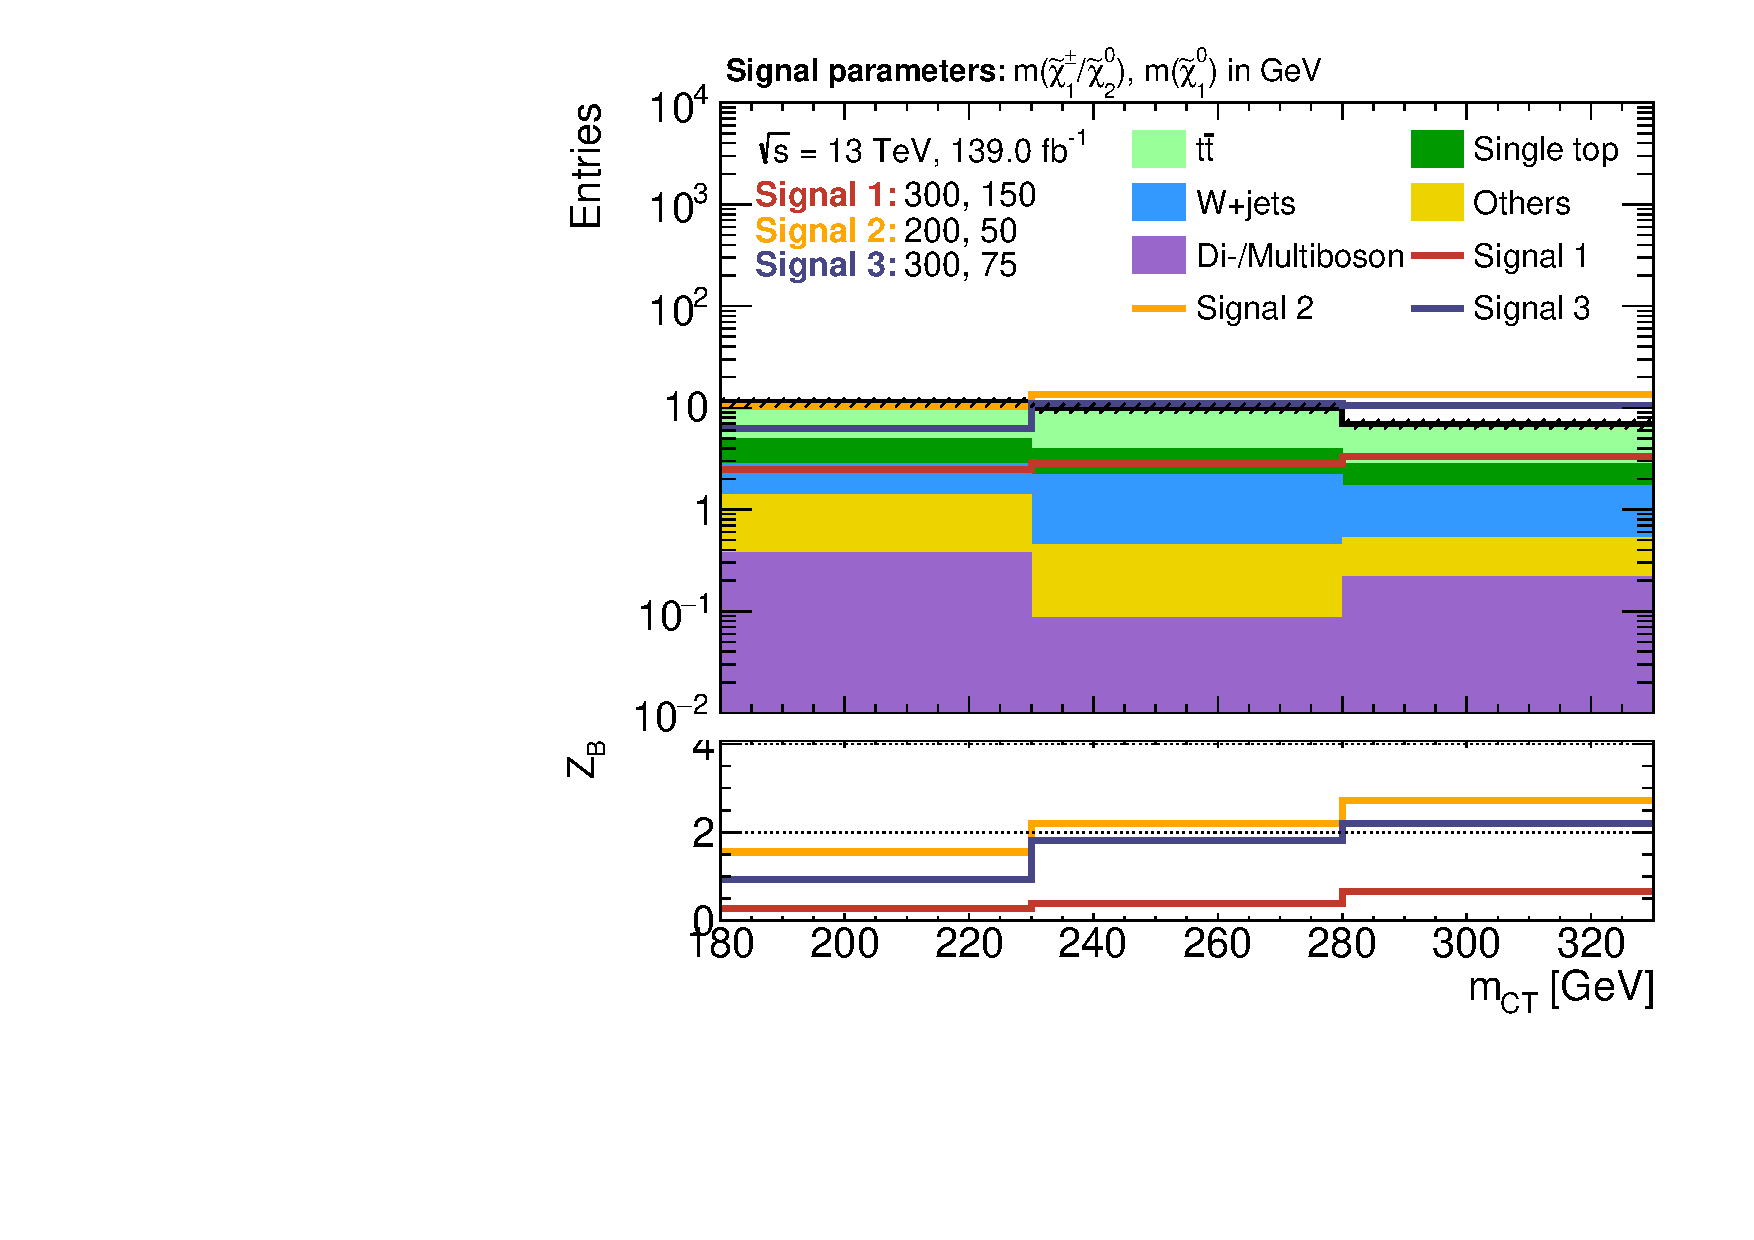
\includegraphics[width=\textwidth]{n1_SRLM_mct_bins/mct.pdf}
		\vspace{-2em}
		\caption{\label{fig:Wh_reopt_second_round_n1_srlm_mct}}
	\end{subfigure}
	\par\medskip
	\begin{subfigure}[b]{0.45\linewidth}
		\centering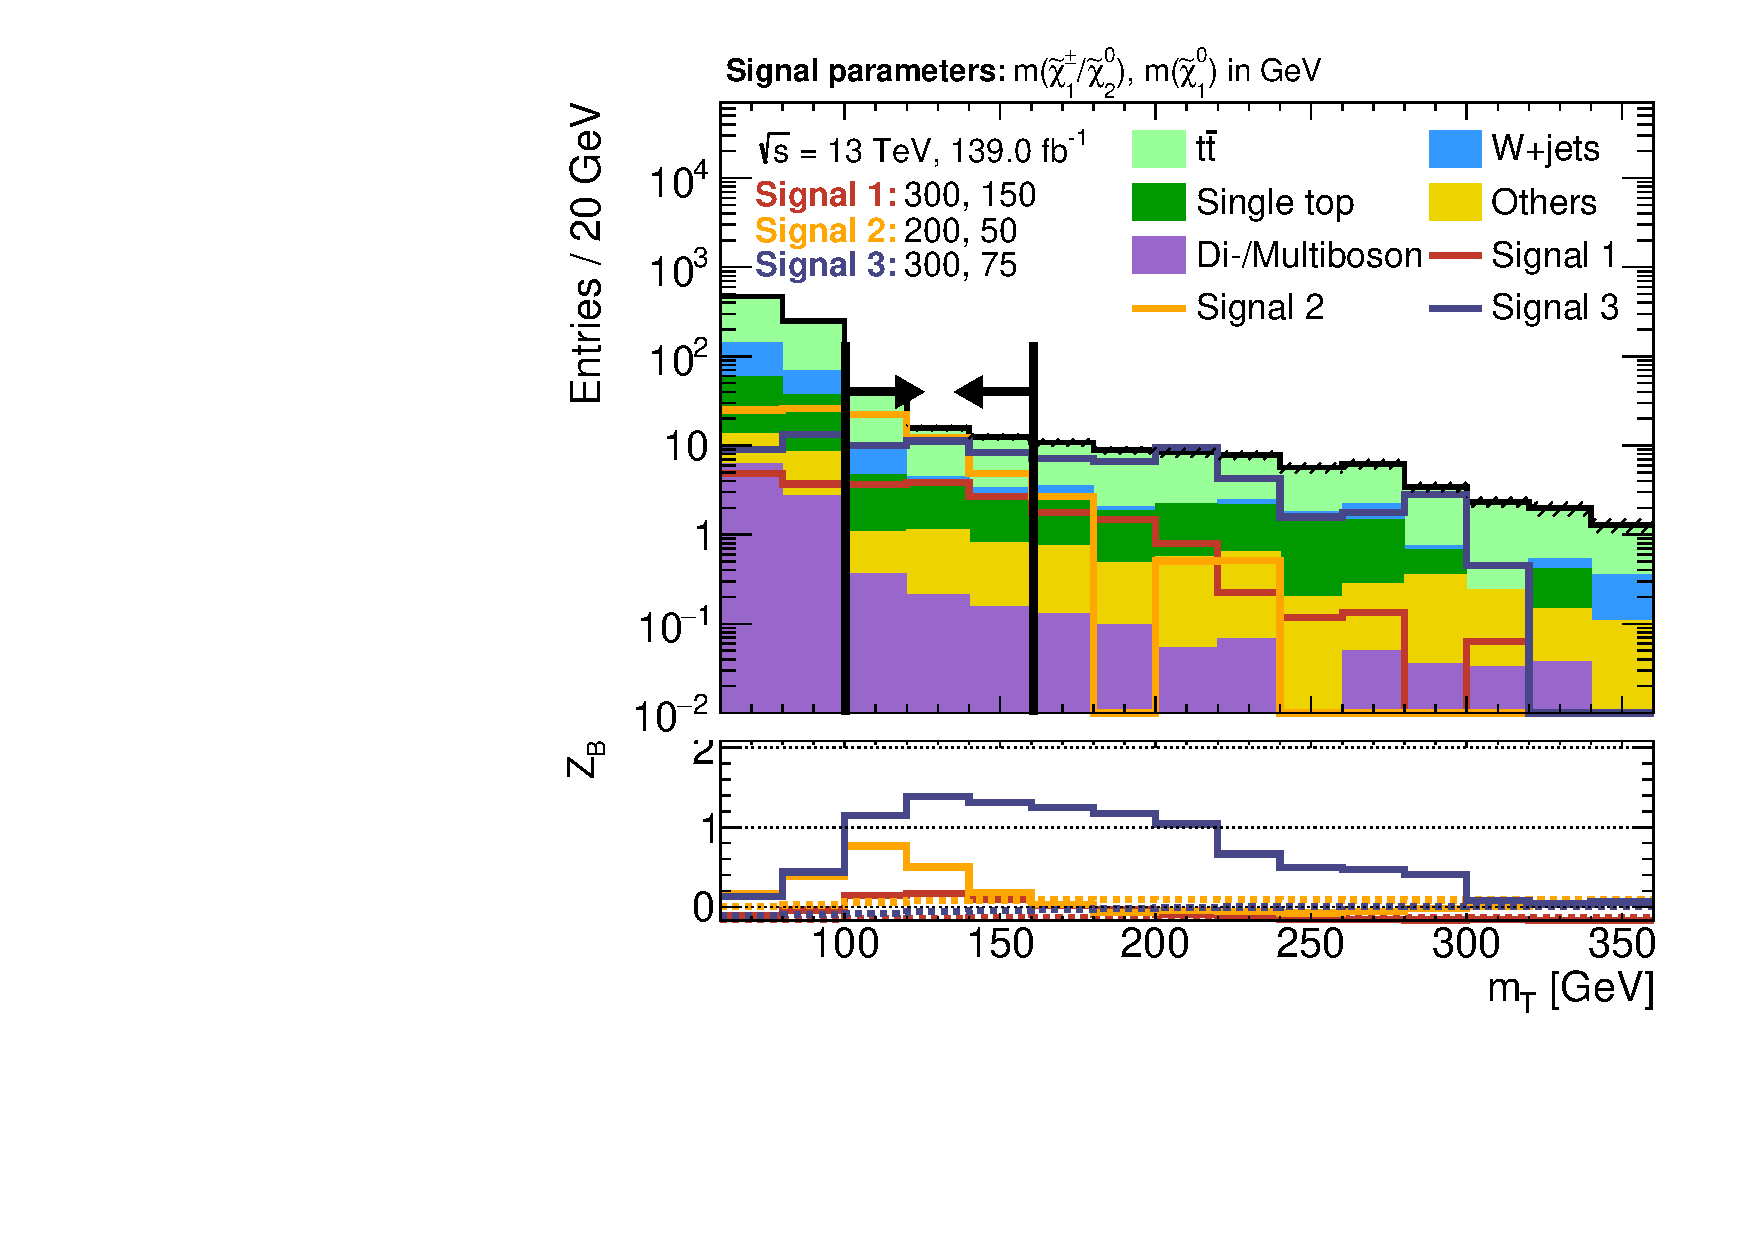
\includegraphics[width=\textwidth]{n1_SRLM_mct_bins/mt_both.pdf}
		\vspace{-2em}
		\caption{\label{fig:Wh_reopt_second_round_n1_srlm_mt}}
	\end{subfigure}%
	\begin{subfigure}[b]{0.45\linewidth}
		\centering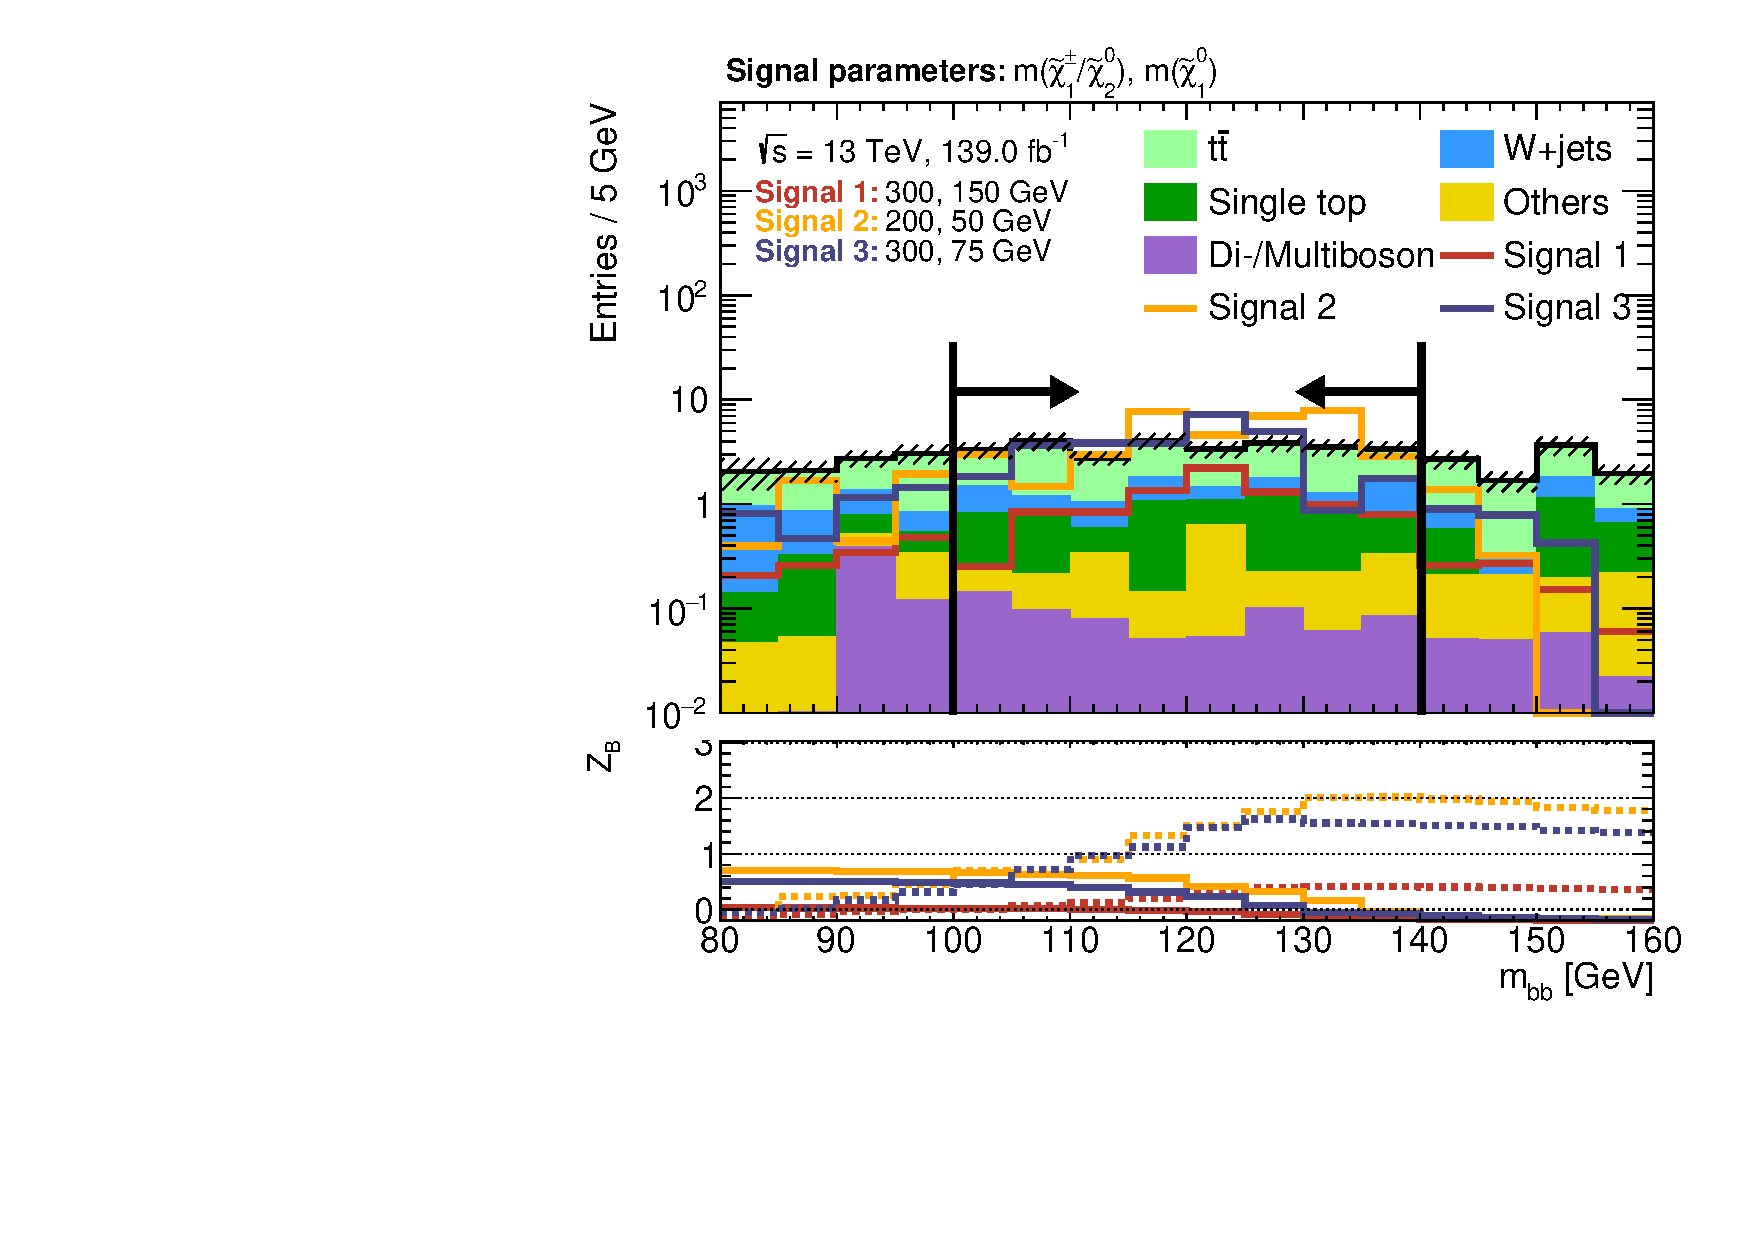
\includegraphics[width=\textwidth]{n1_SRLM_mct_bins/mbb_both.pdf}
		\vspace{-2em}
		\caption{\label{fig:Wh_reopt_second_round_n1_srlm_mbb}}
	\end{subfigure}
%	\begin{subfigure}[b]{0.4\linewidth}
%		\centering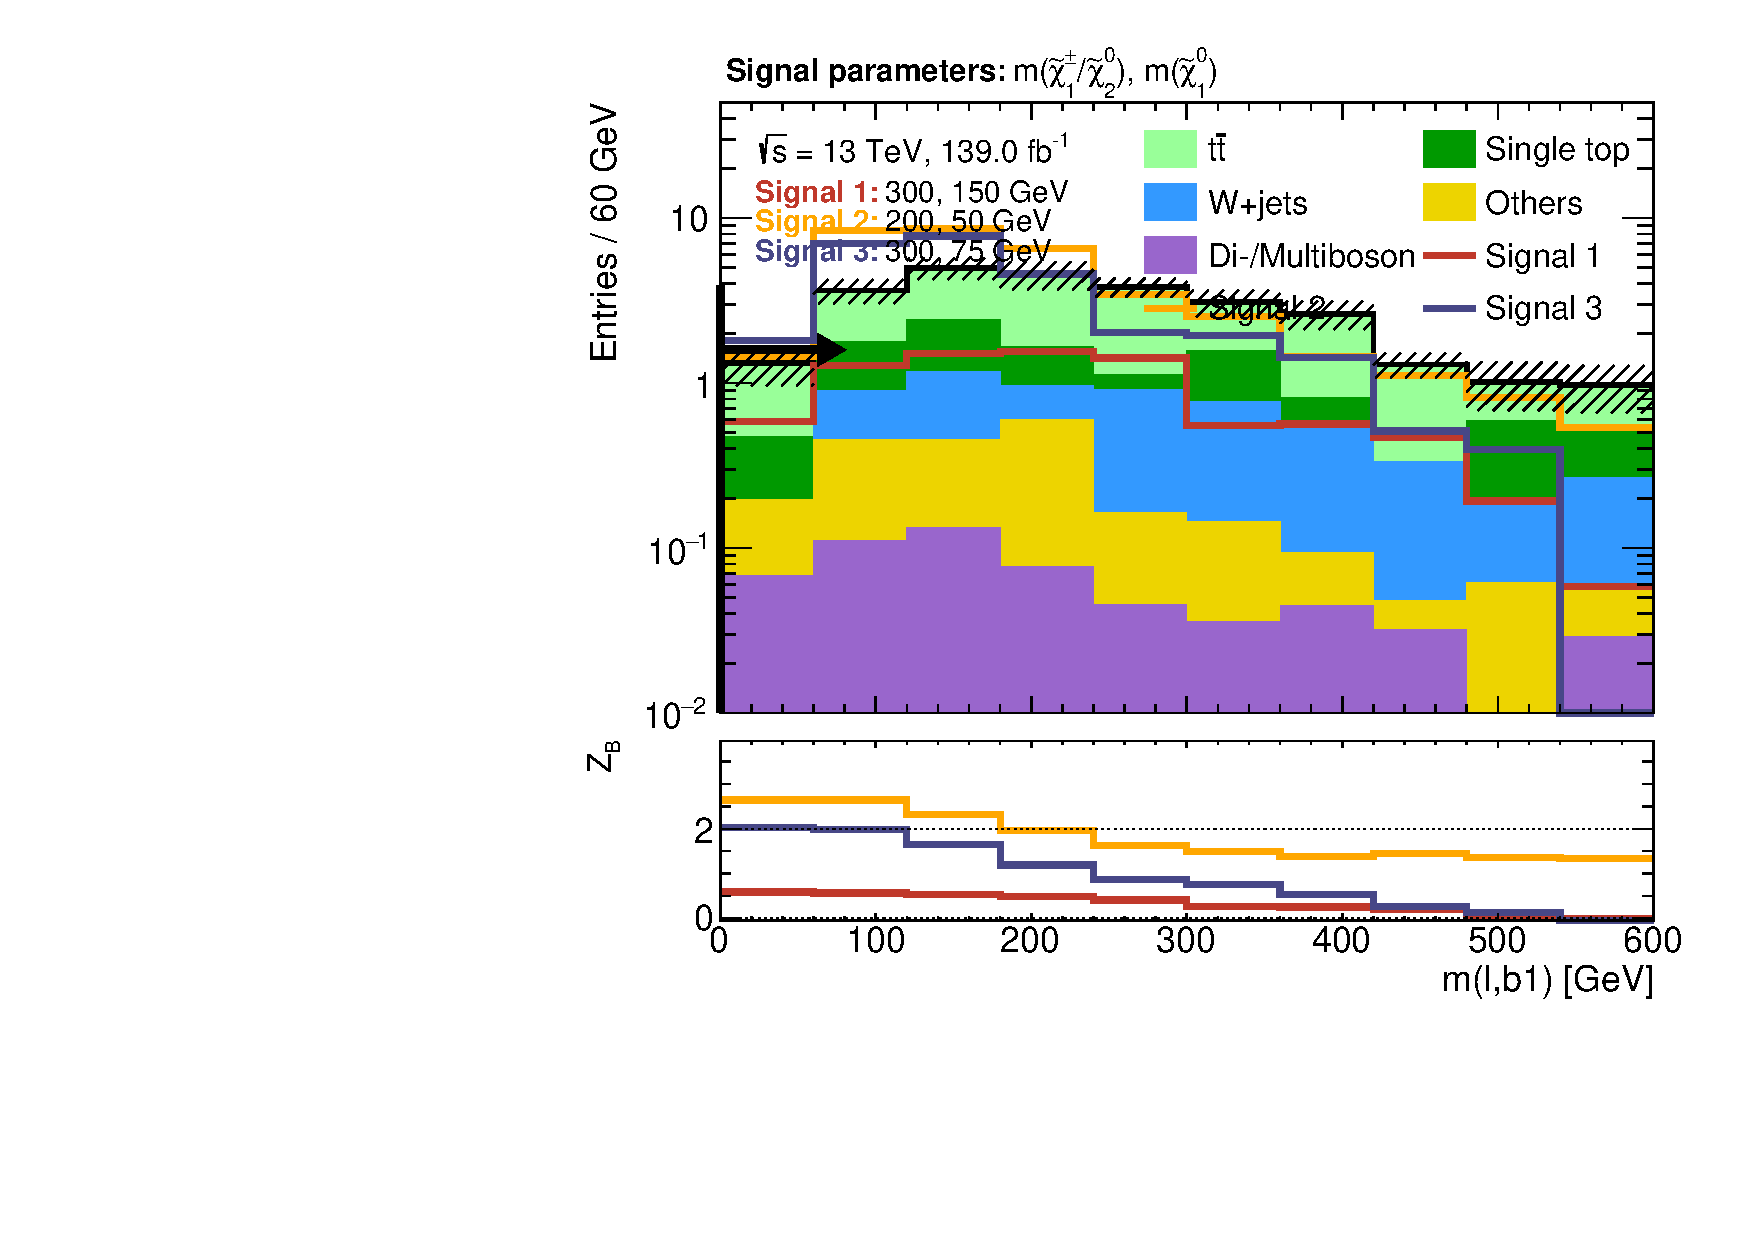
\includegraphics[width=\textwidth]{n1_SRLM_mct_bins/mlb1.pdf}
%		\caption{\label{fig:Wh_reopt_second_round_n1_srlm_mlb1}}
%	\end{subfigure}%
	\par\medskip
	\begin{subfigure}[b]{0.45\linewidth}
		\centering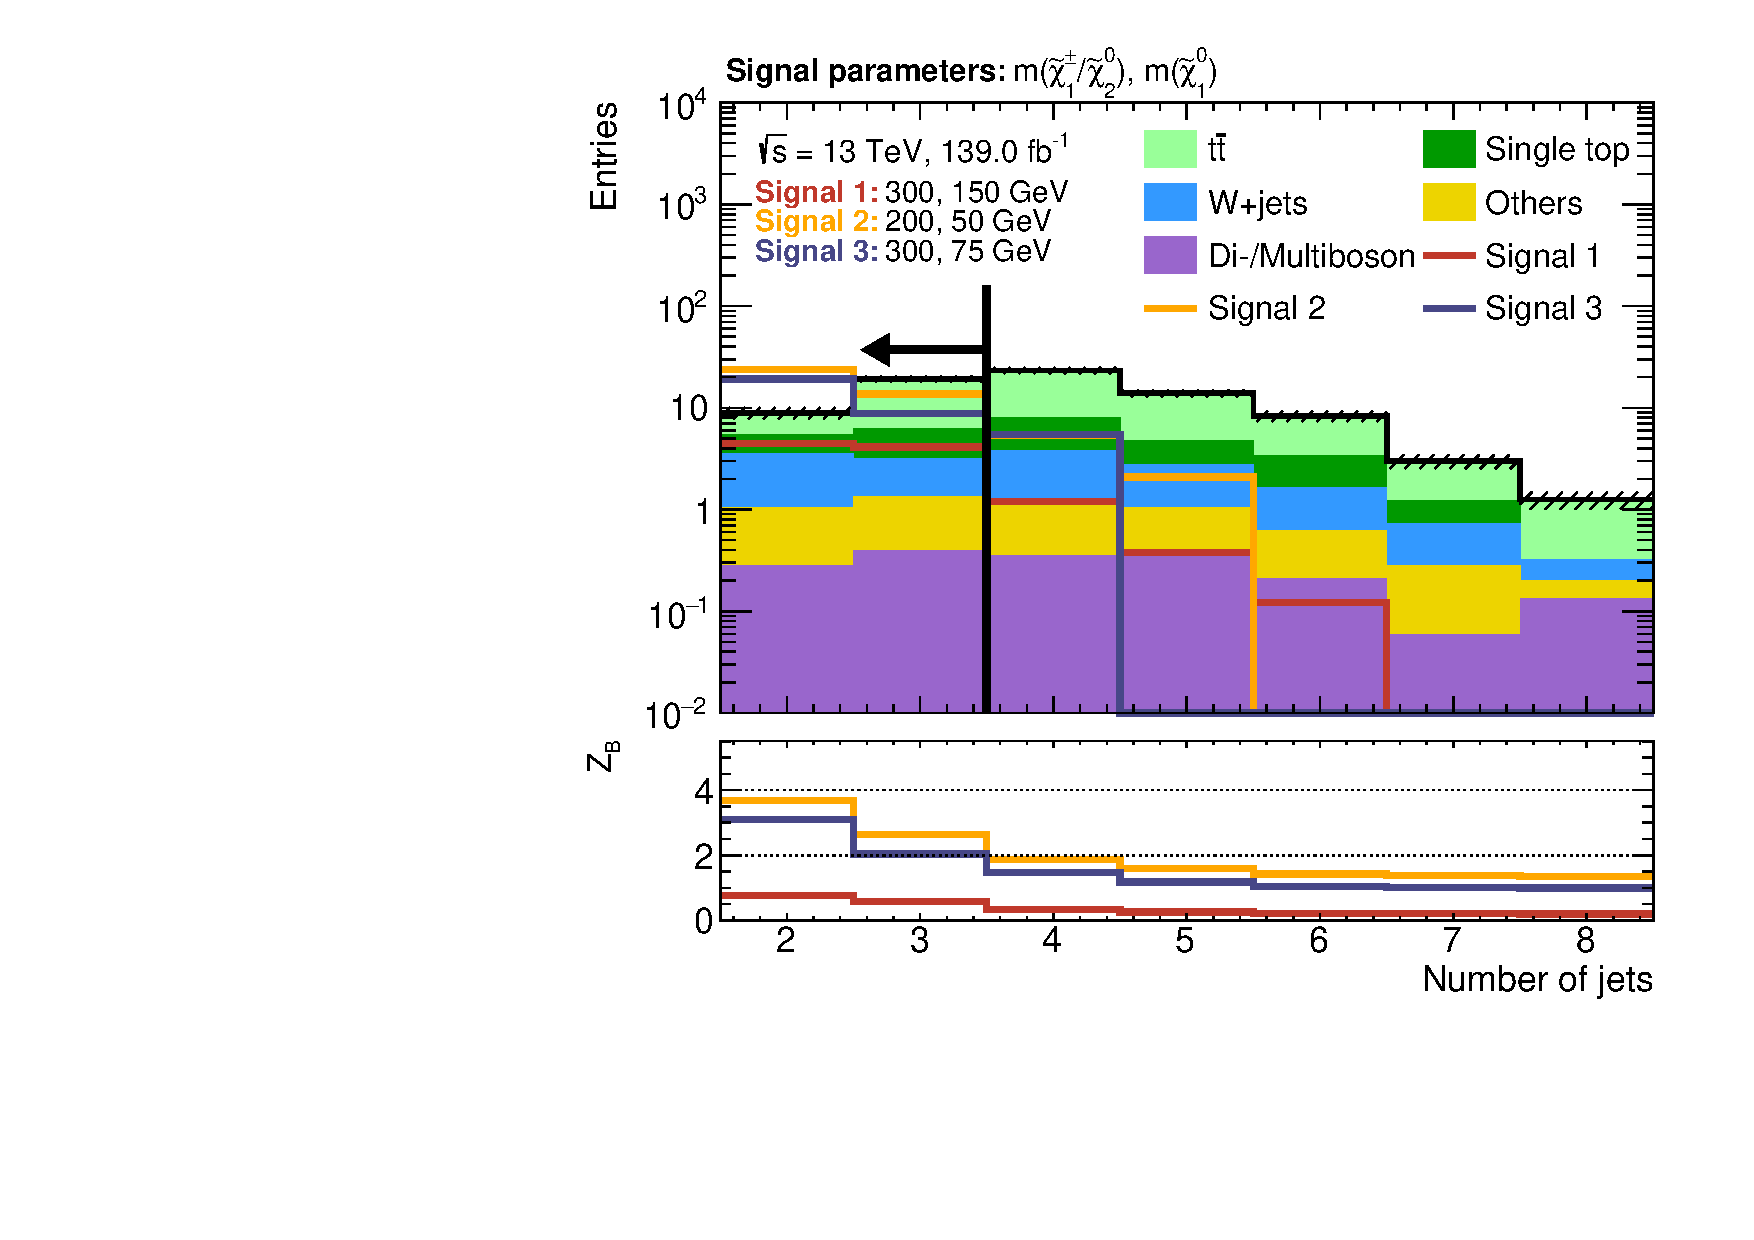
\includegraphics[width=\textwidth]{n1_SRLM_mct_bins/nJet30.pdf}
		\vspace{-2em}
		\caption{\label{fig:Wh_reopt_second_round_n1_srlm_njet}}
	\end{subfigure}
	\caption{\textit{N}--1 plots for SR-LM, with representative signal points and all $\mct$ bins included. The dashed area represents the \gls{mc} statistical uncertainties on the background. In all figures except \figname~\subref{fig:Wh_reopt_second_round_n1_srlm_mct}, the significance in the lower pad is obtained by summing up all the events in the direction of the cut arrow and includes 30\% systematic uncertainties as well as MC statistical uncertainties. In \figname~\subref{fig:Wh_reopt_second_round_n1_srlm_mct} the significance is only computed on a bin-by-bin basis, \ie not summing up all events in the direction of the cut arrow.}
	\label{fig:Wh_reopt_second_round_n1_srlm}
\end{figure}

\begin{figure}
	\centering
	\begin{subfigure}[b]{0.45\linewidth}
		\centering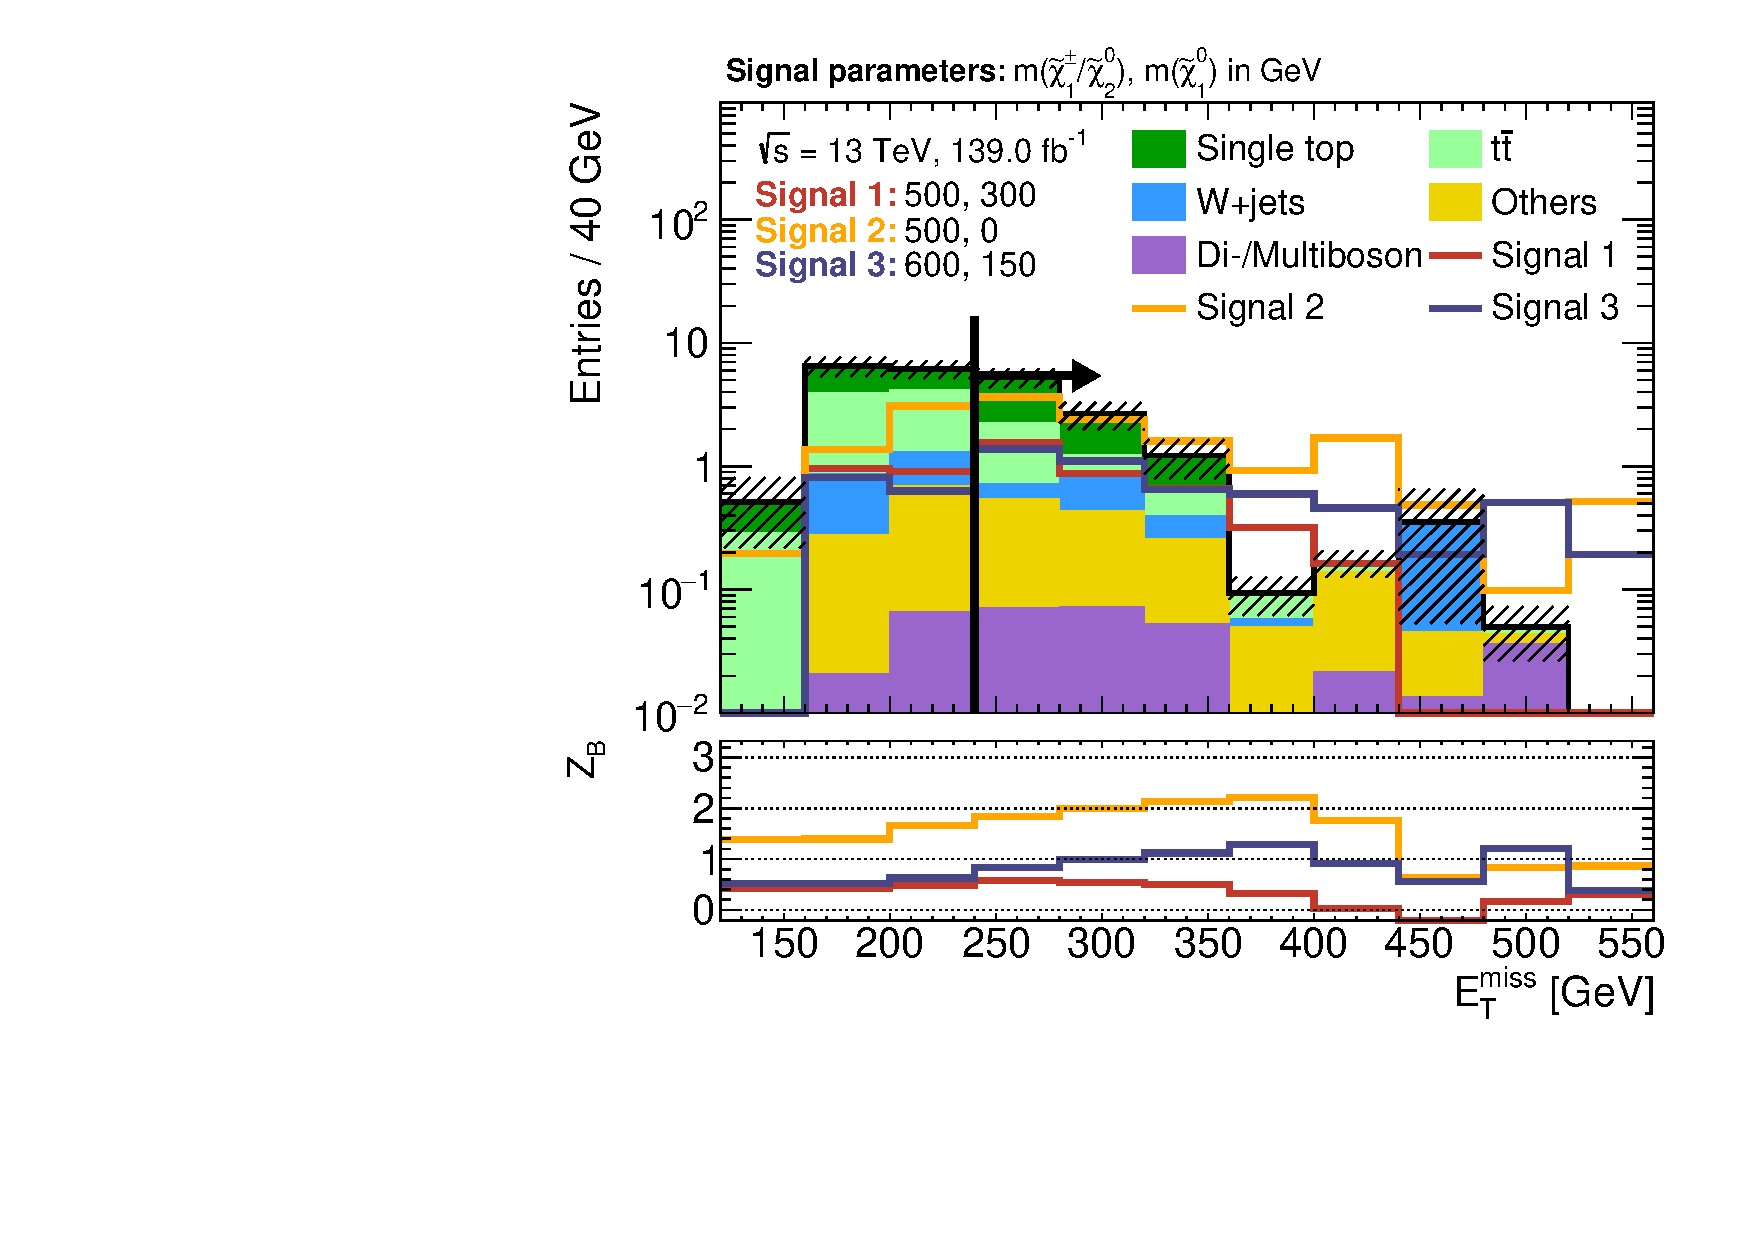
\includegraphics[width=\textwidth]{n1_SRMM_mct_bins/met.pdf}
		\vspace{-2em}
		\caption{\label{fig:Wh_reopt_second_round_n1_srmm_met}}
	\end{subfigure}%
	\begin{subfigure}[b]{0.45\linewidth}
		\centering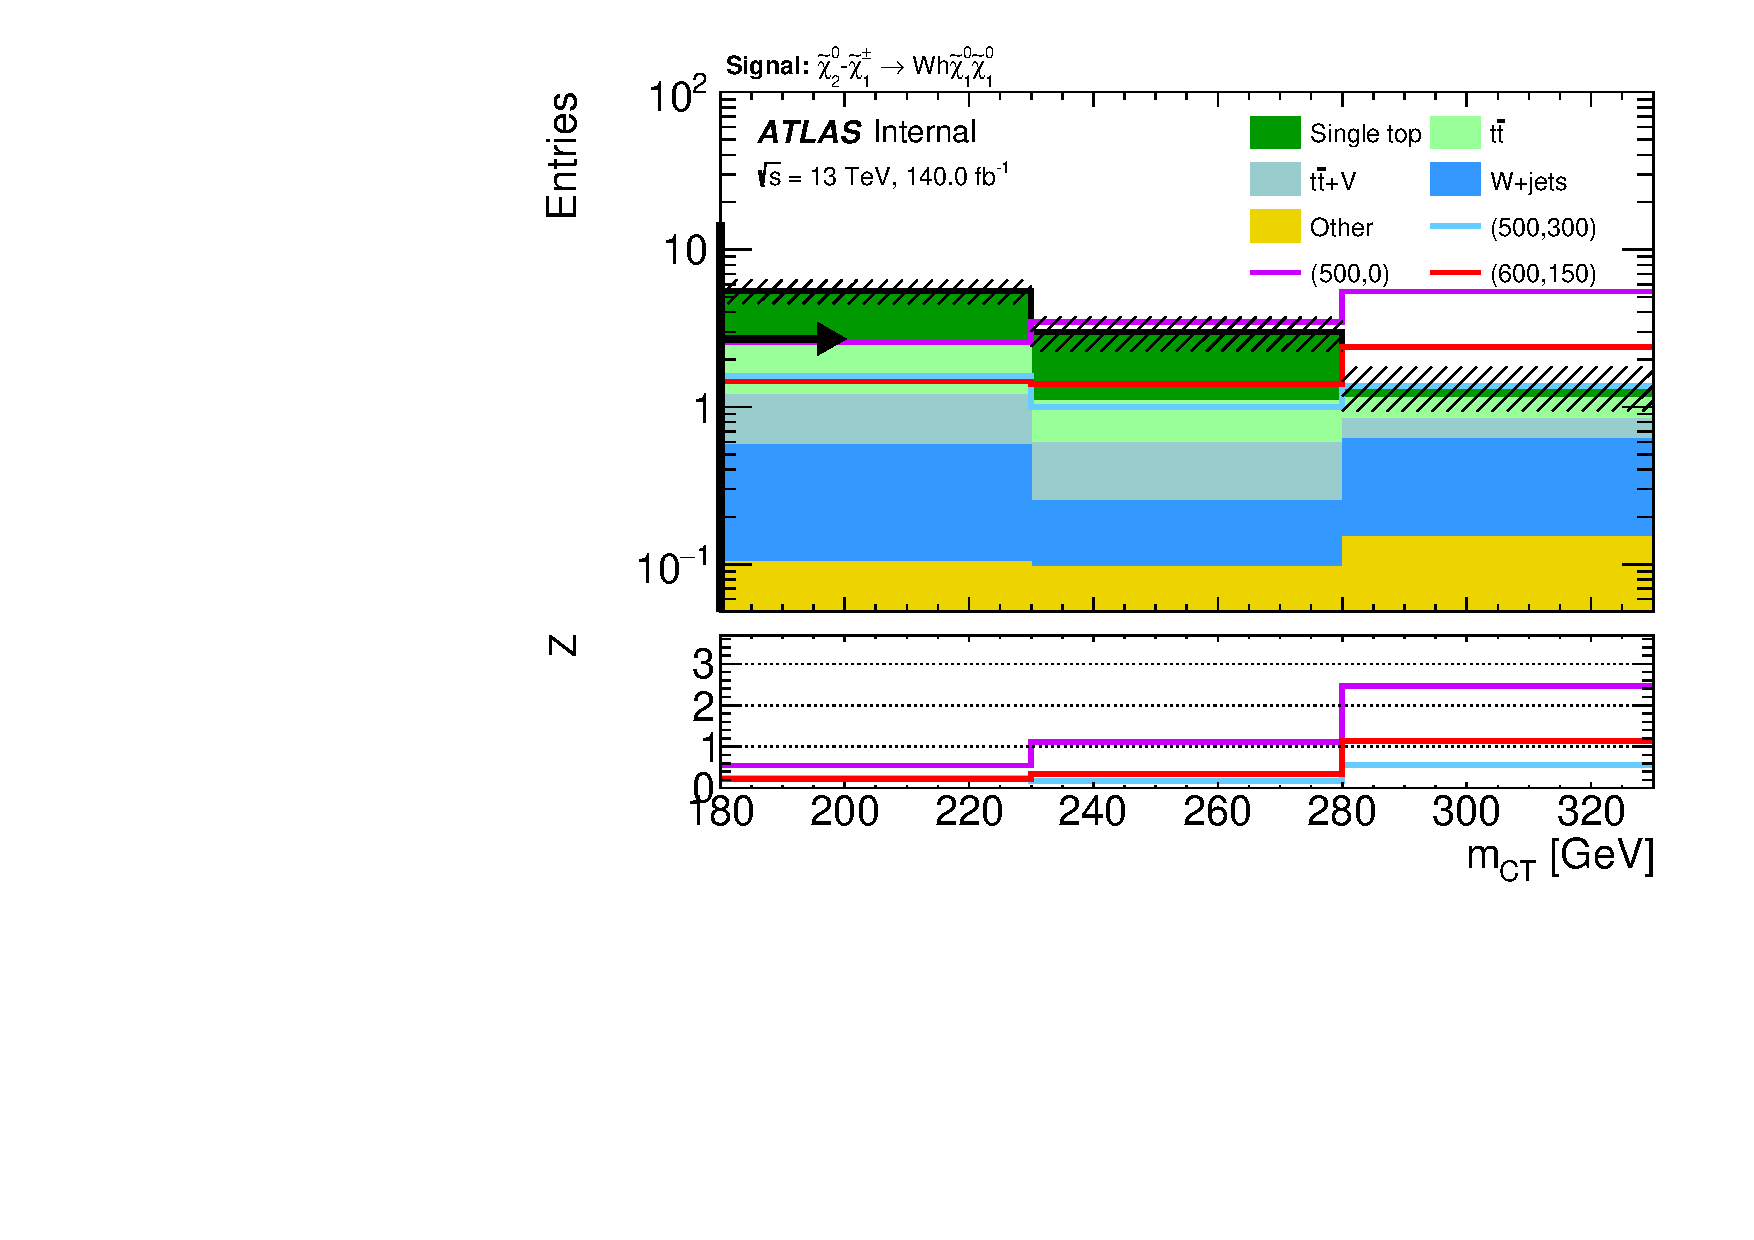
\includegraphics[width=\textwidth]{n1_SRMM_mct_bins/mct.pdf}
		\vspace{-2em}
		\caption{\label{fig:Wh_reopt_second_round_n1_srmm_mct}}
	\end{subfigure}
	\par\medskip
	\begin{subfigure}[b]{0.45\linewidth}
		\centering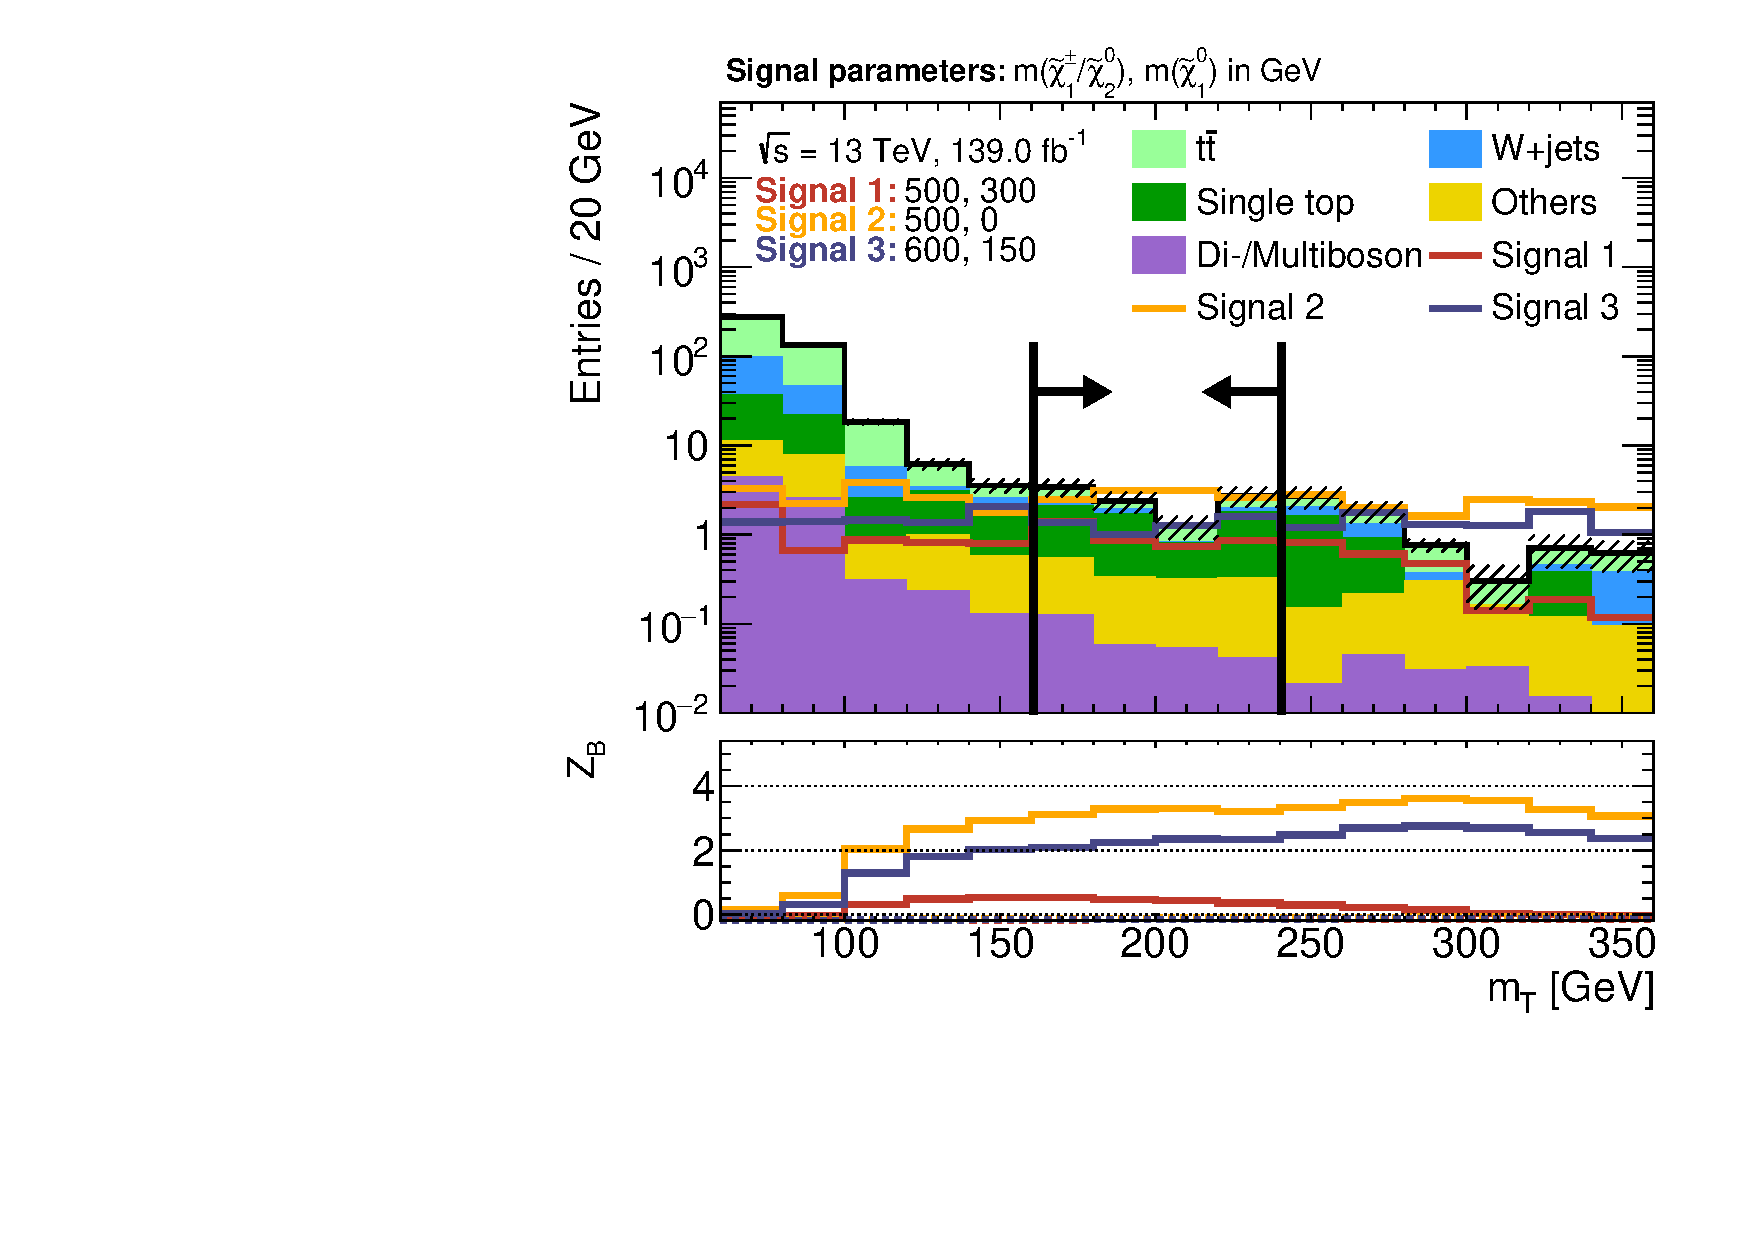
\includegraphics[width=\textwidth]{n1_SRMM_mct_bins/mt_both.pdf}
		\vspace{-2em}
		\caption{\label{fig:Wh_reopt_second_round_n1_srmm_mt}}
	\end{subfigure}%
	\begin{subfigure}[b]{0.45\linewidth}
		\centering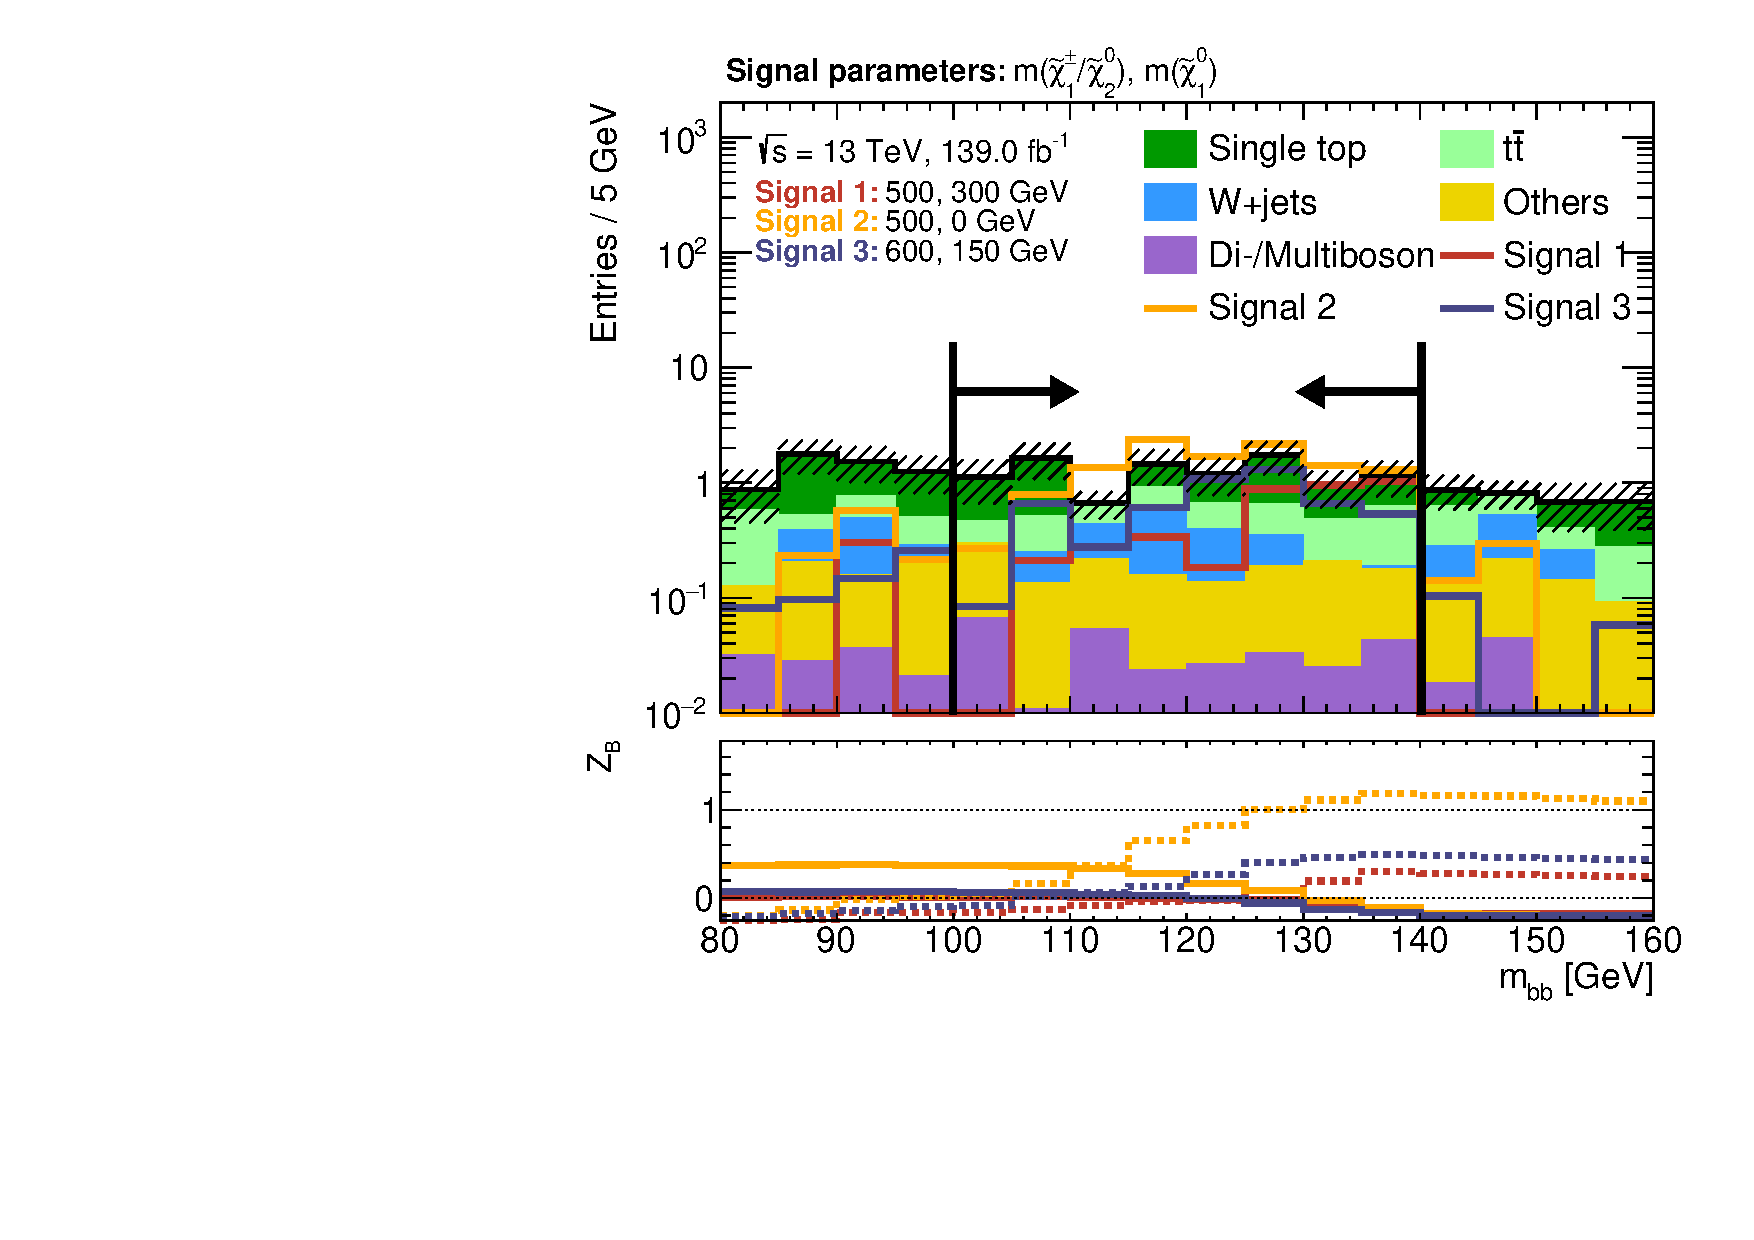
\includegraphics[width=\textwidth]{n1_SRMM_mct_bins/mbb_both.pdf}
		\vspace{-2em}
		\caption{\label{fig:Wh_reopt_second_round_n1_srmm_mbb}}
	\end{subfigure}
%	\begin{subfigure}[b]{0.4\linewidth}
%		\centering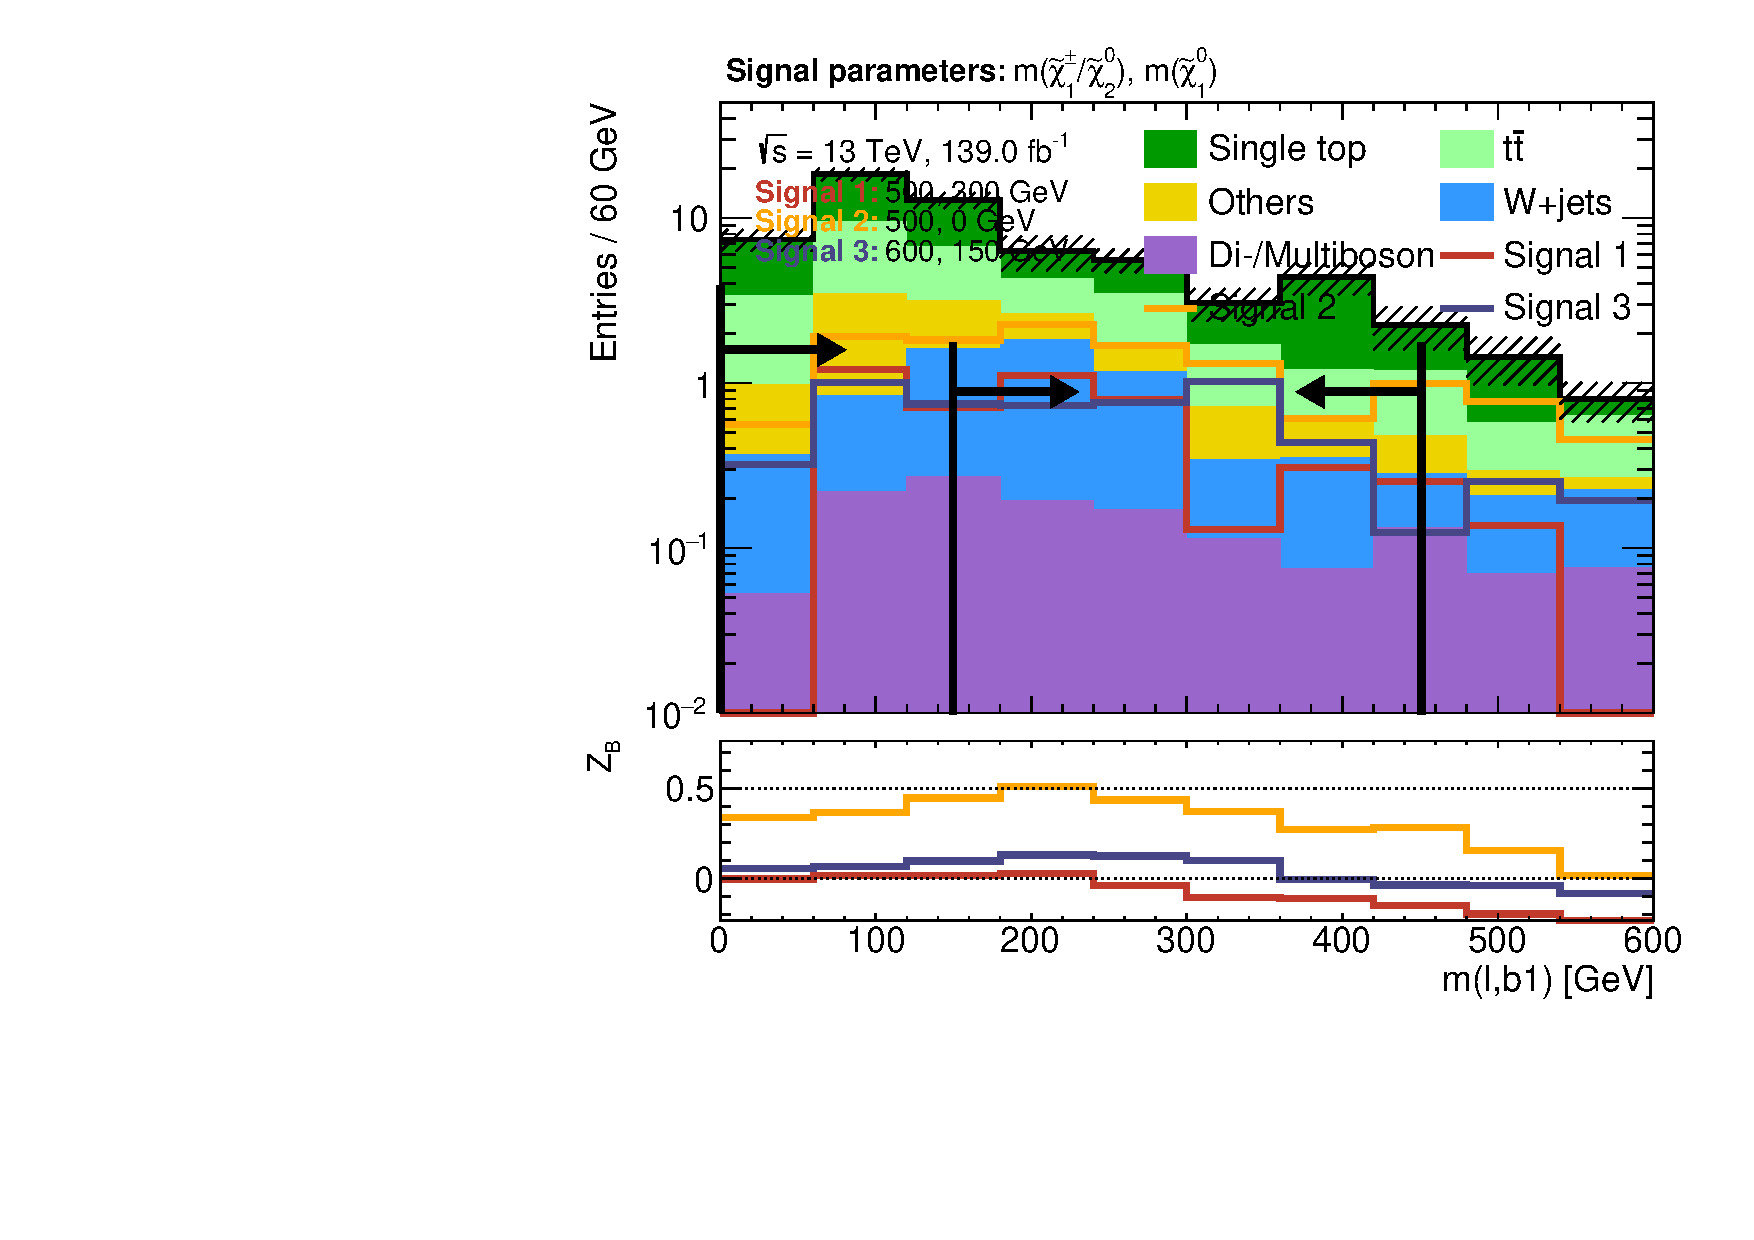
\includegraphics[width=\textwidth]{n1_SRMM_mct_bins/mlb1.pdf}
%		\caption{\label{fig:Wh_reopt_second_round_n1_srmm_mlb1}}
%	\end{subfigure}%
	\par\medskip
	\begin{subfigure}[b]{0.45\linewidth}
		\centering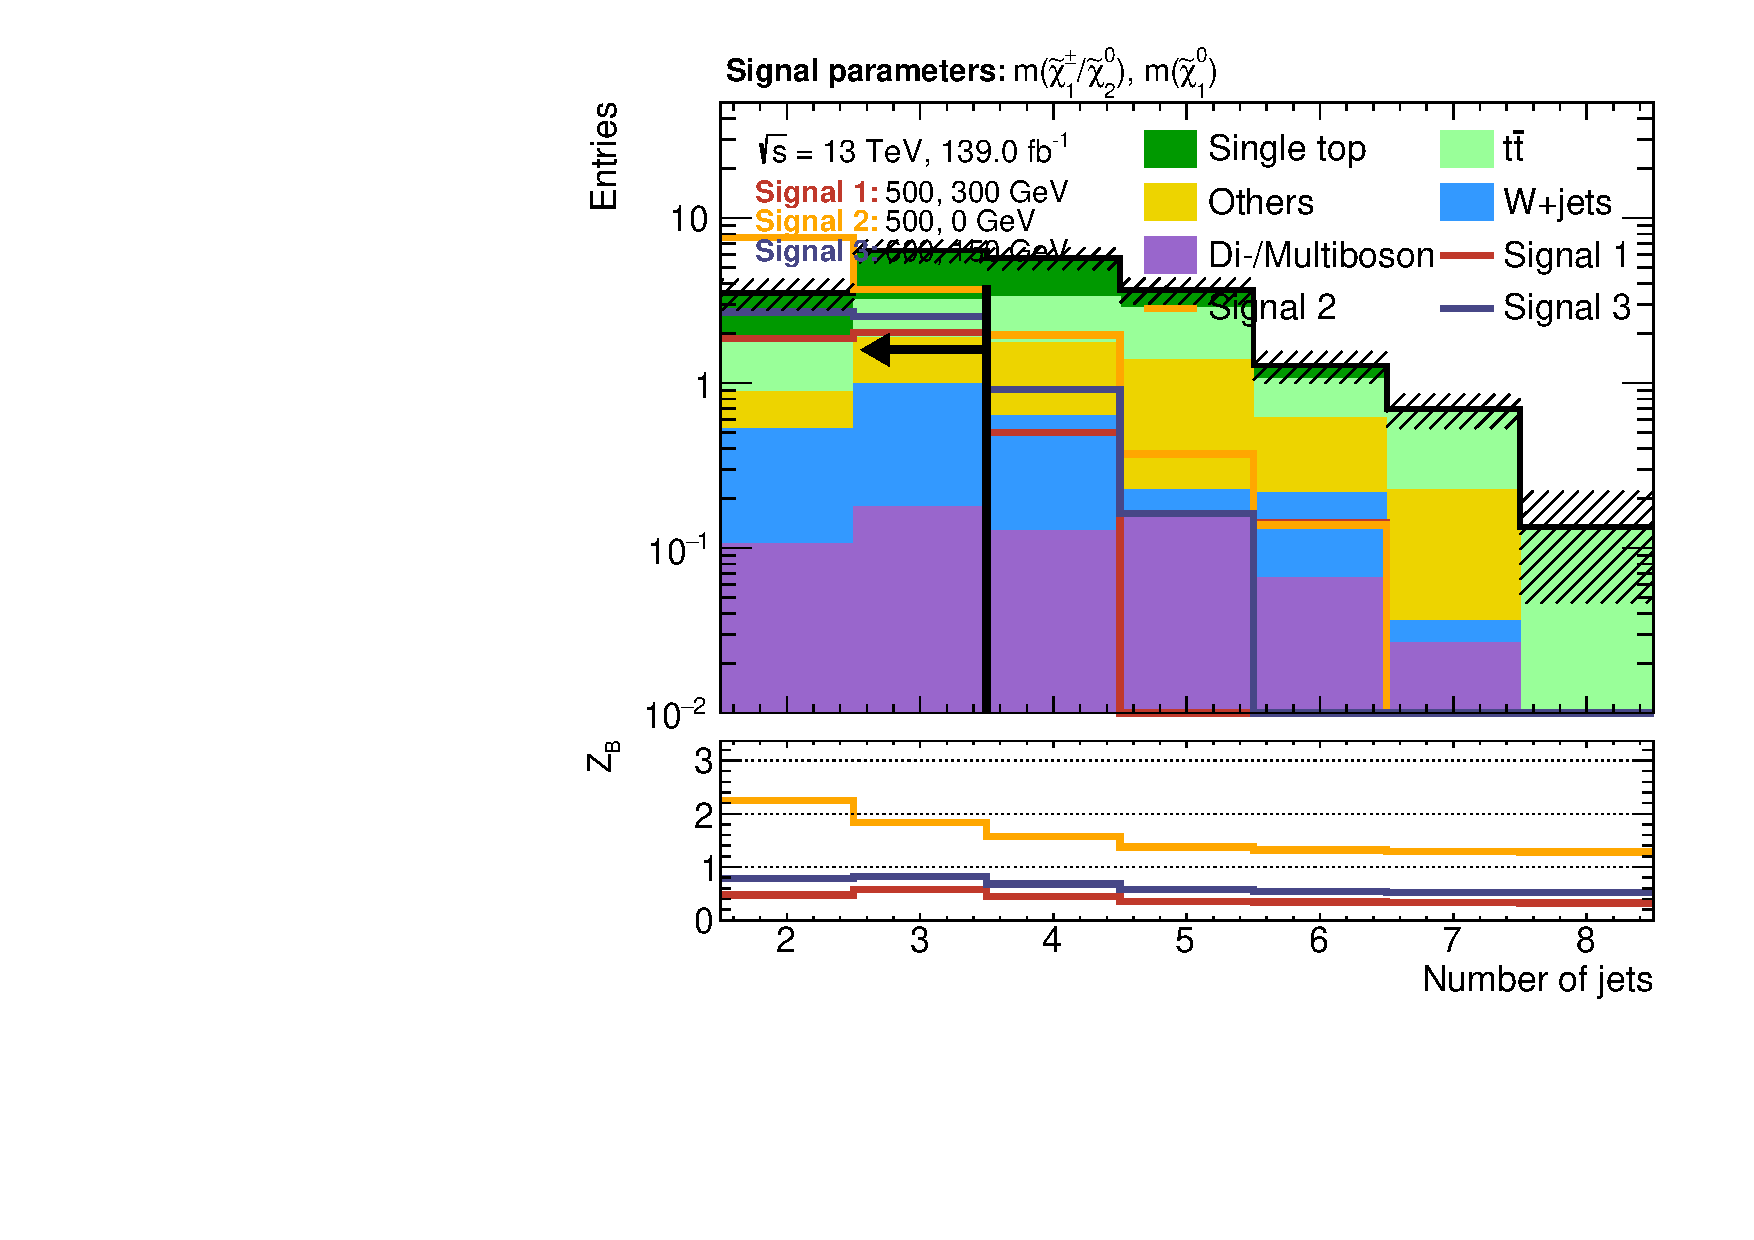
\includegraphics[width=\textwidth]{n1_SRMM_mct_bins/nJet30.pdf}
		\vspace{-2em}
		\caption{\label{fig:Wh_reopt_second_round_n1_srmm_njet}}
	\end{subfigure}
	\caption{\textit{N}--1 plots for SR-MM, with representative signal points and all $\mct$ bins included. The dashed area represents the \gls{mc} statistical uncertainties on the background. In all figures except \figname~\subref{fig:Wh_reopt_second_round_n1_srmm_mct}, the significance in the lower pad is obtained by summing up all the events in the direction of the cut arrow and includes 30\% systematic uncertainties as well as MC statistical uncertainties. In \figname~\subref{fig:Wh_reopt_second_round_n1_srmm_mct} the significance is only computed on a bin-by-bin basis, \ie not summing up all events in the direction of the cut arrow.}
	\label{fig:Wh_reopt_second_round_n1_srmm}
\end{figure}

\begin{figure}
	\centering
	\begin{subfigure}[b]{0.45\linewidth}
		\centering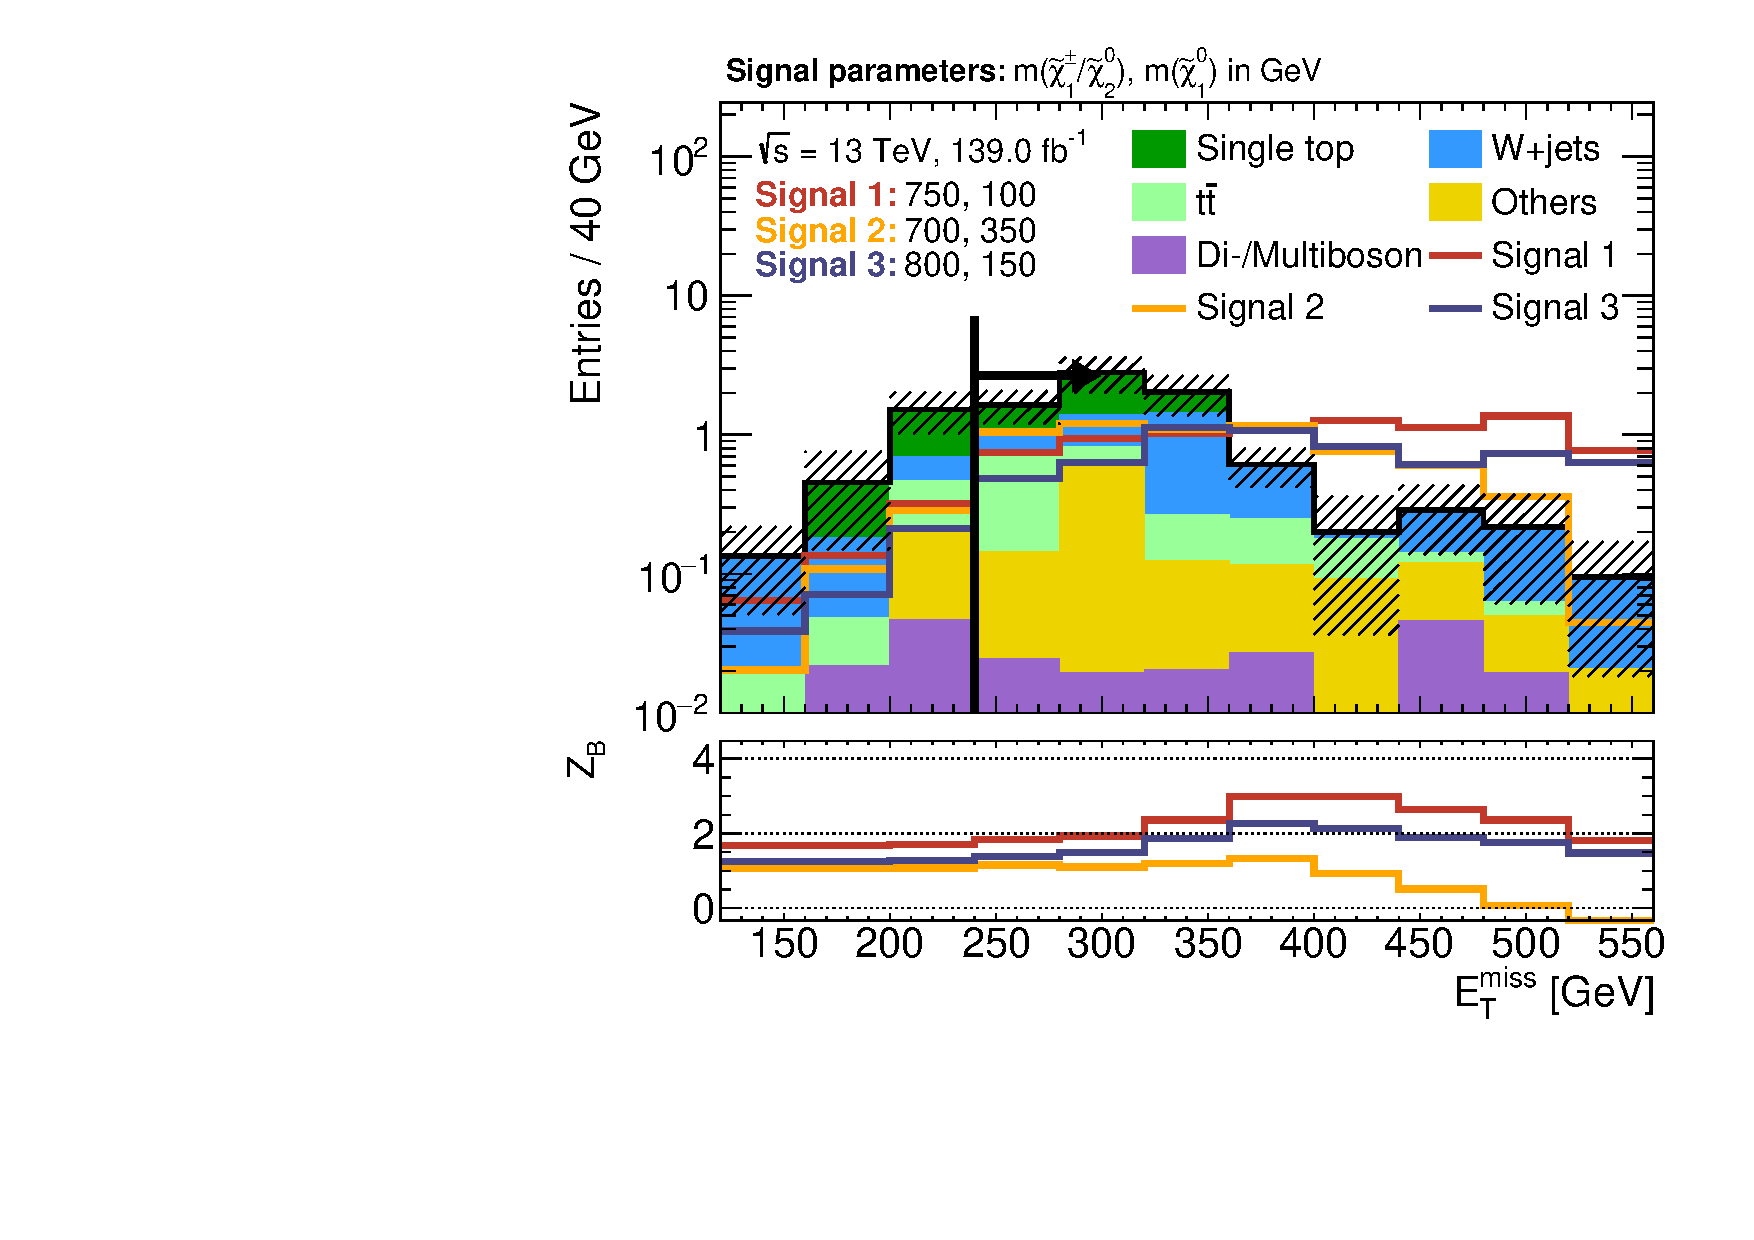
\includegraphics[width=\textwidth]{n1_SRHM_mct_bins/met.pdf}
		\vspace{-2em}
		\caption{\label{fig:Wh_reopt_second_round_n1_srhm_met}}
	\end{subfigure}%
	\begin{subfigure}[b]{0.45\linewidth}
		\centering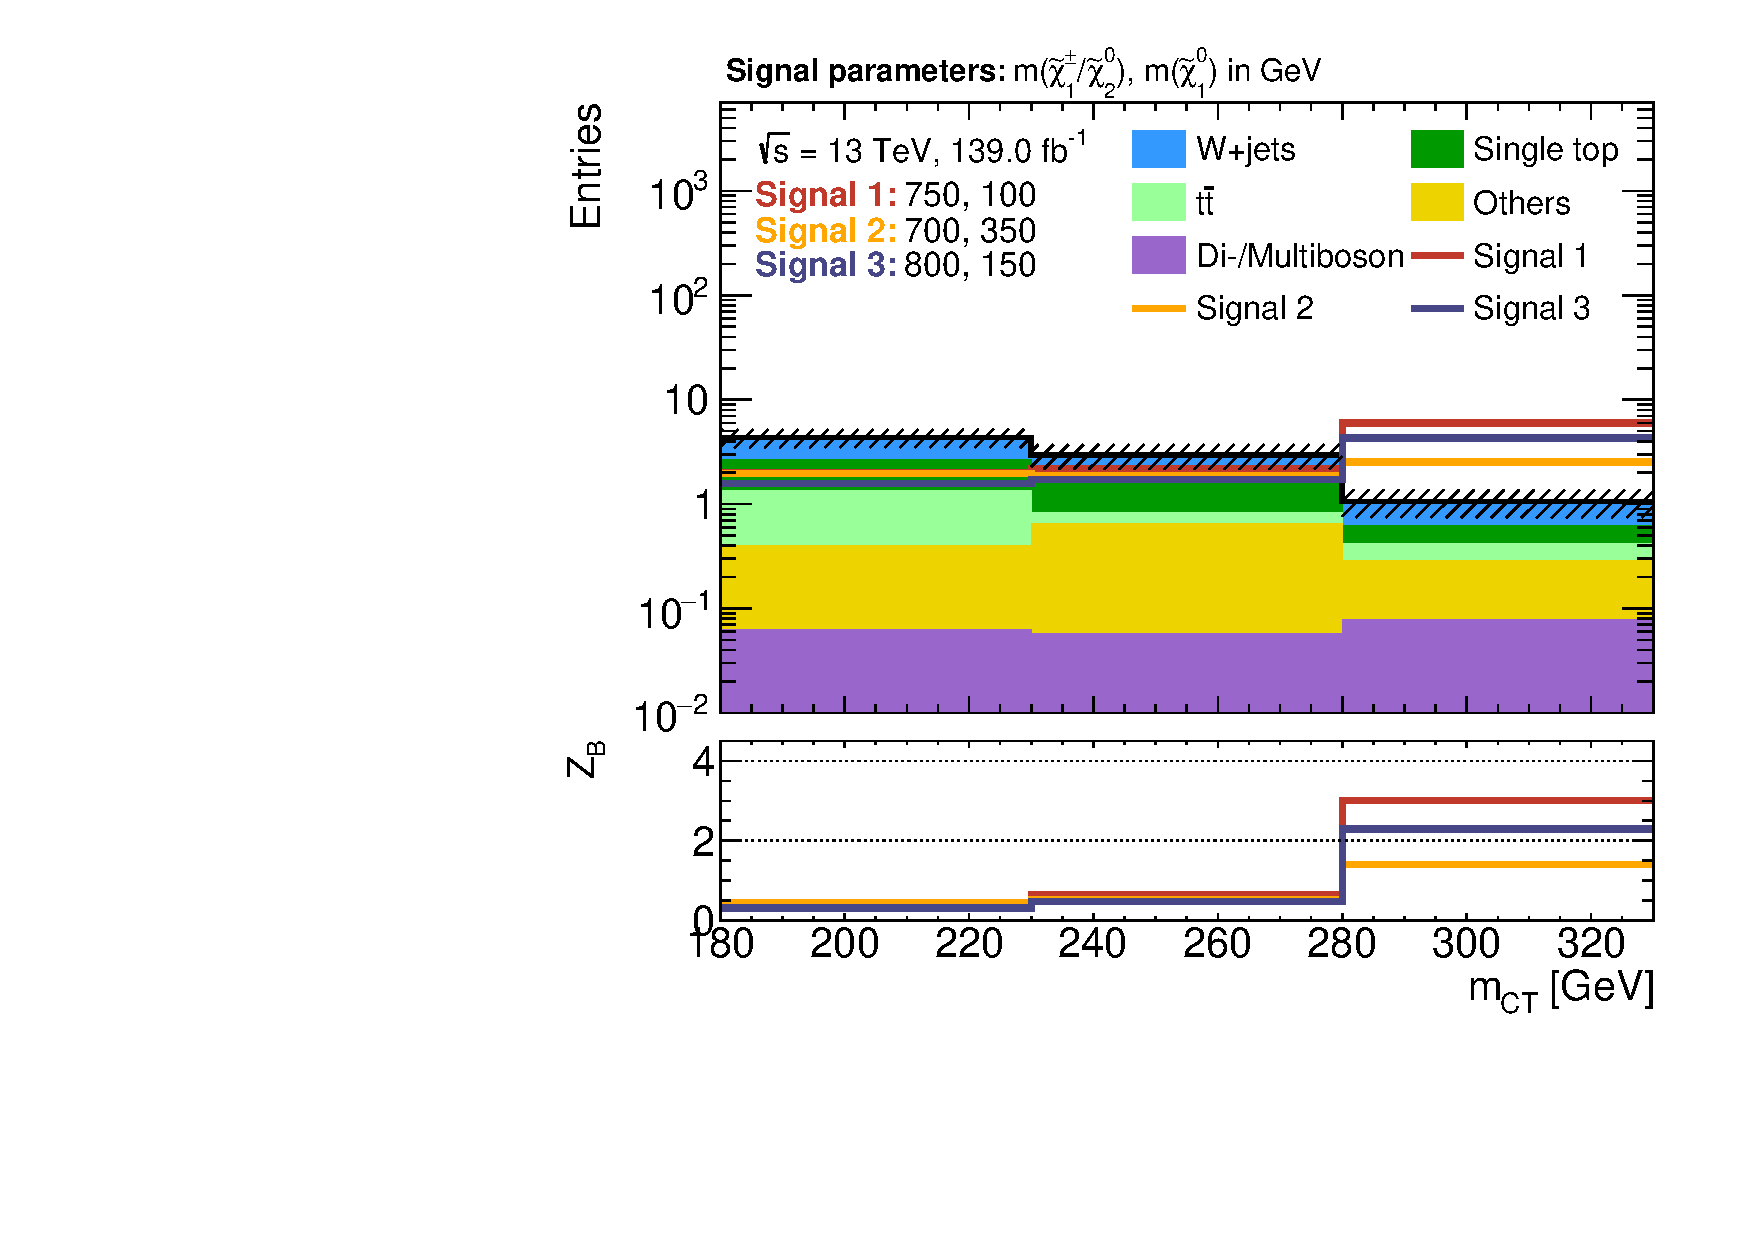
\includegraphics[width=\textwidth]{n1_SRHM_mct_bins/mct.pdf}
		\vspace{-2em}
		\caption{\label{fig:Wh_reopt_second_round_n1_srhm_mct}}
	\end{subfigure}
	\par\medskip
	\begin{subfigure}[b]{0.45\linewidth}
		\centering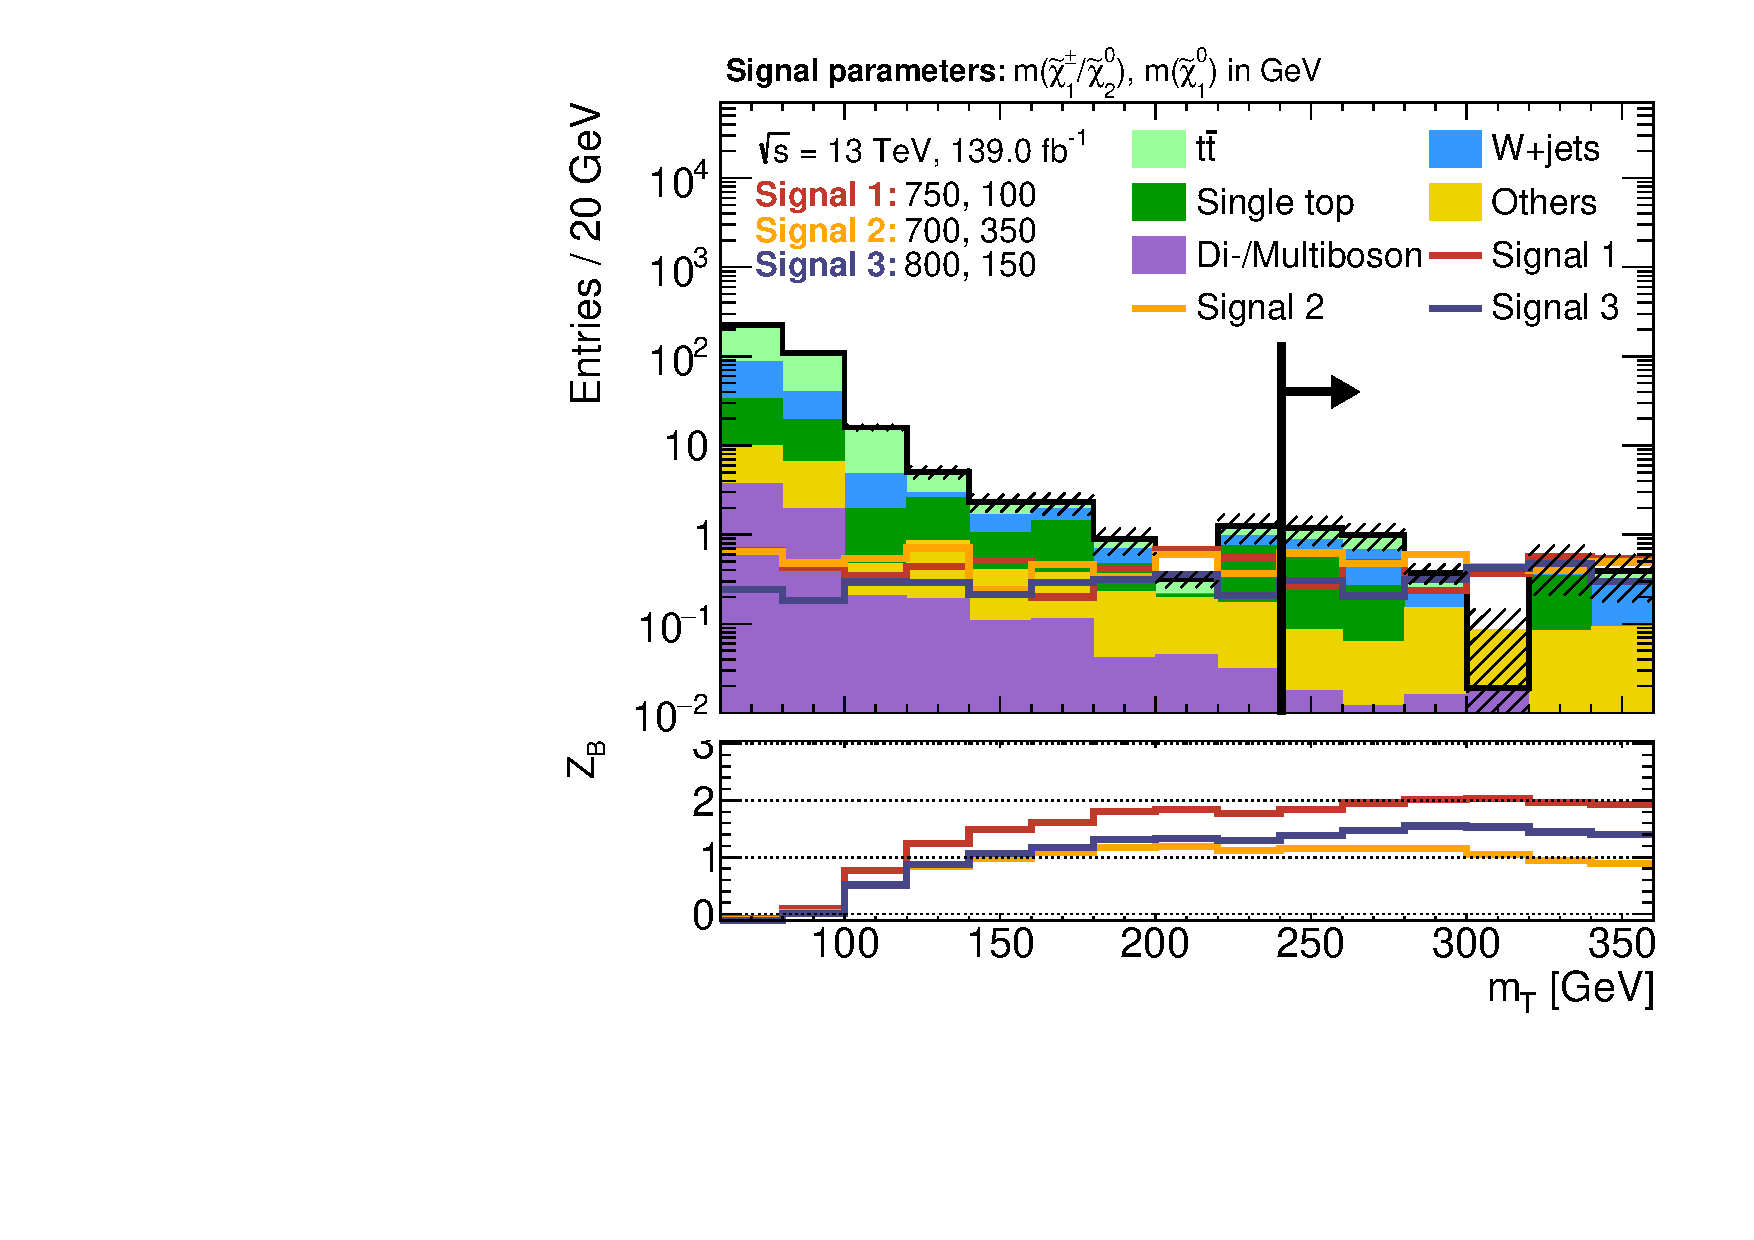
\includegraphics[width=\textwidth]{n1_SRHM_mct_bins/mt_both.pdf}
		\vspace{-2em}
		\caption{\label{fig:Wh_reopt_second_round_n1_srhm_mt}}
	\end{subfigure}%
	\begin{subfigure}[b]{0.45\linewidth}
		\centering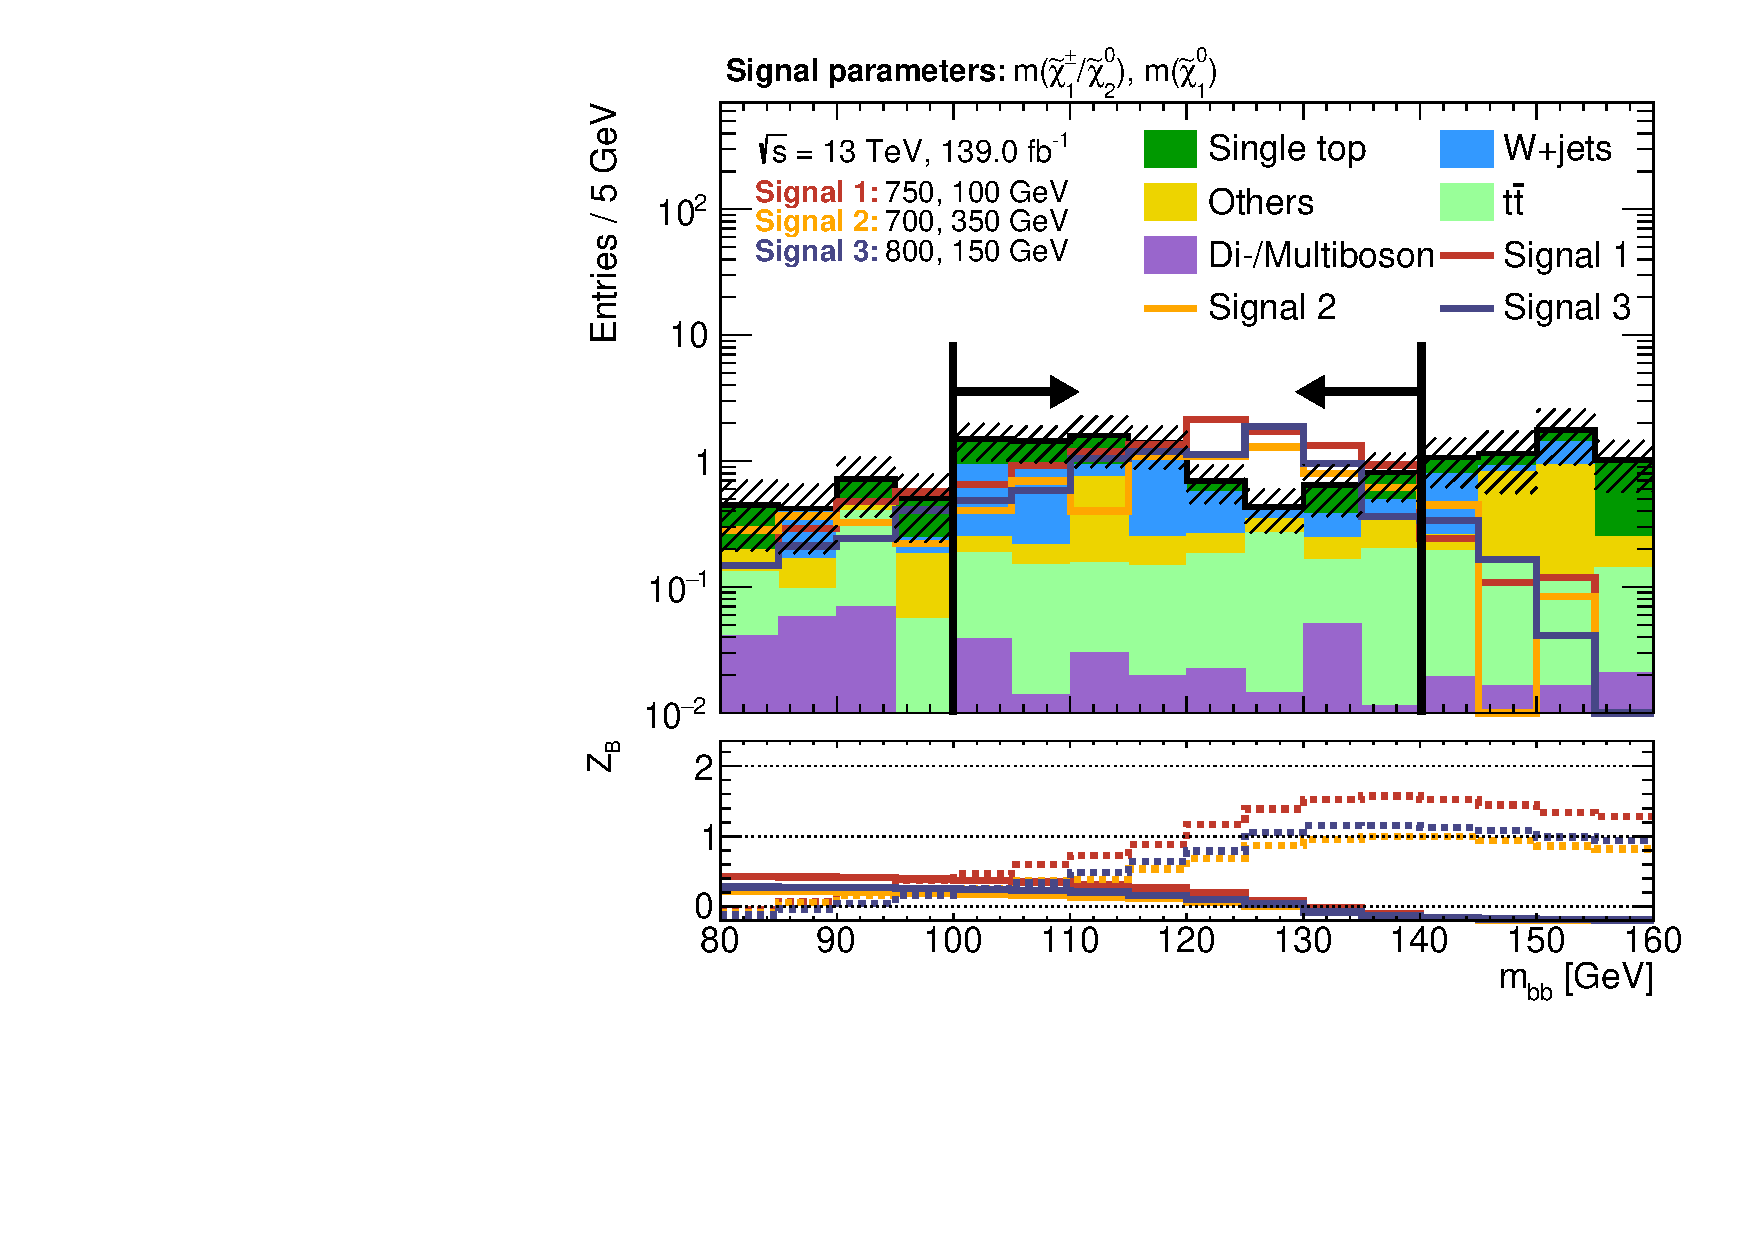
\includegraphics[width=\textwidth]{n1_SRHM_mct_bins/mbb_both.pdf}
		\vspace{-2em}
		\caption{\label{fig:Wh_reopt_second_round_n1_srhm_mbb}}
	\end{subfigure}
	\par\medskip
	\begin{subfigure}[b]{0.45\linewidth}
		\centering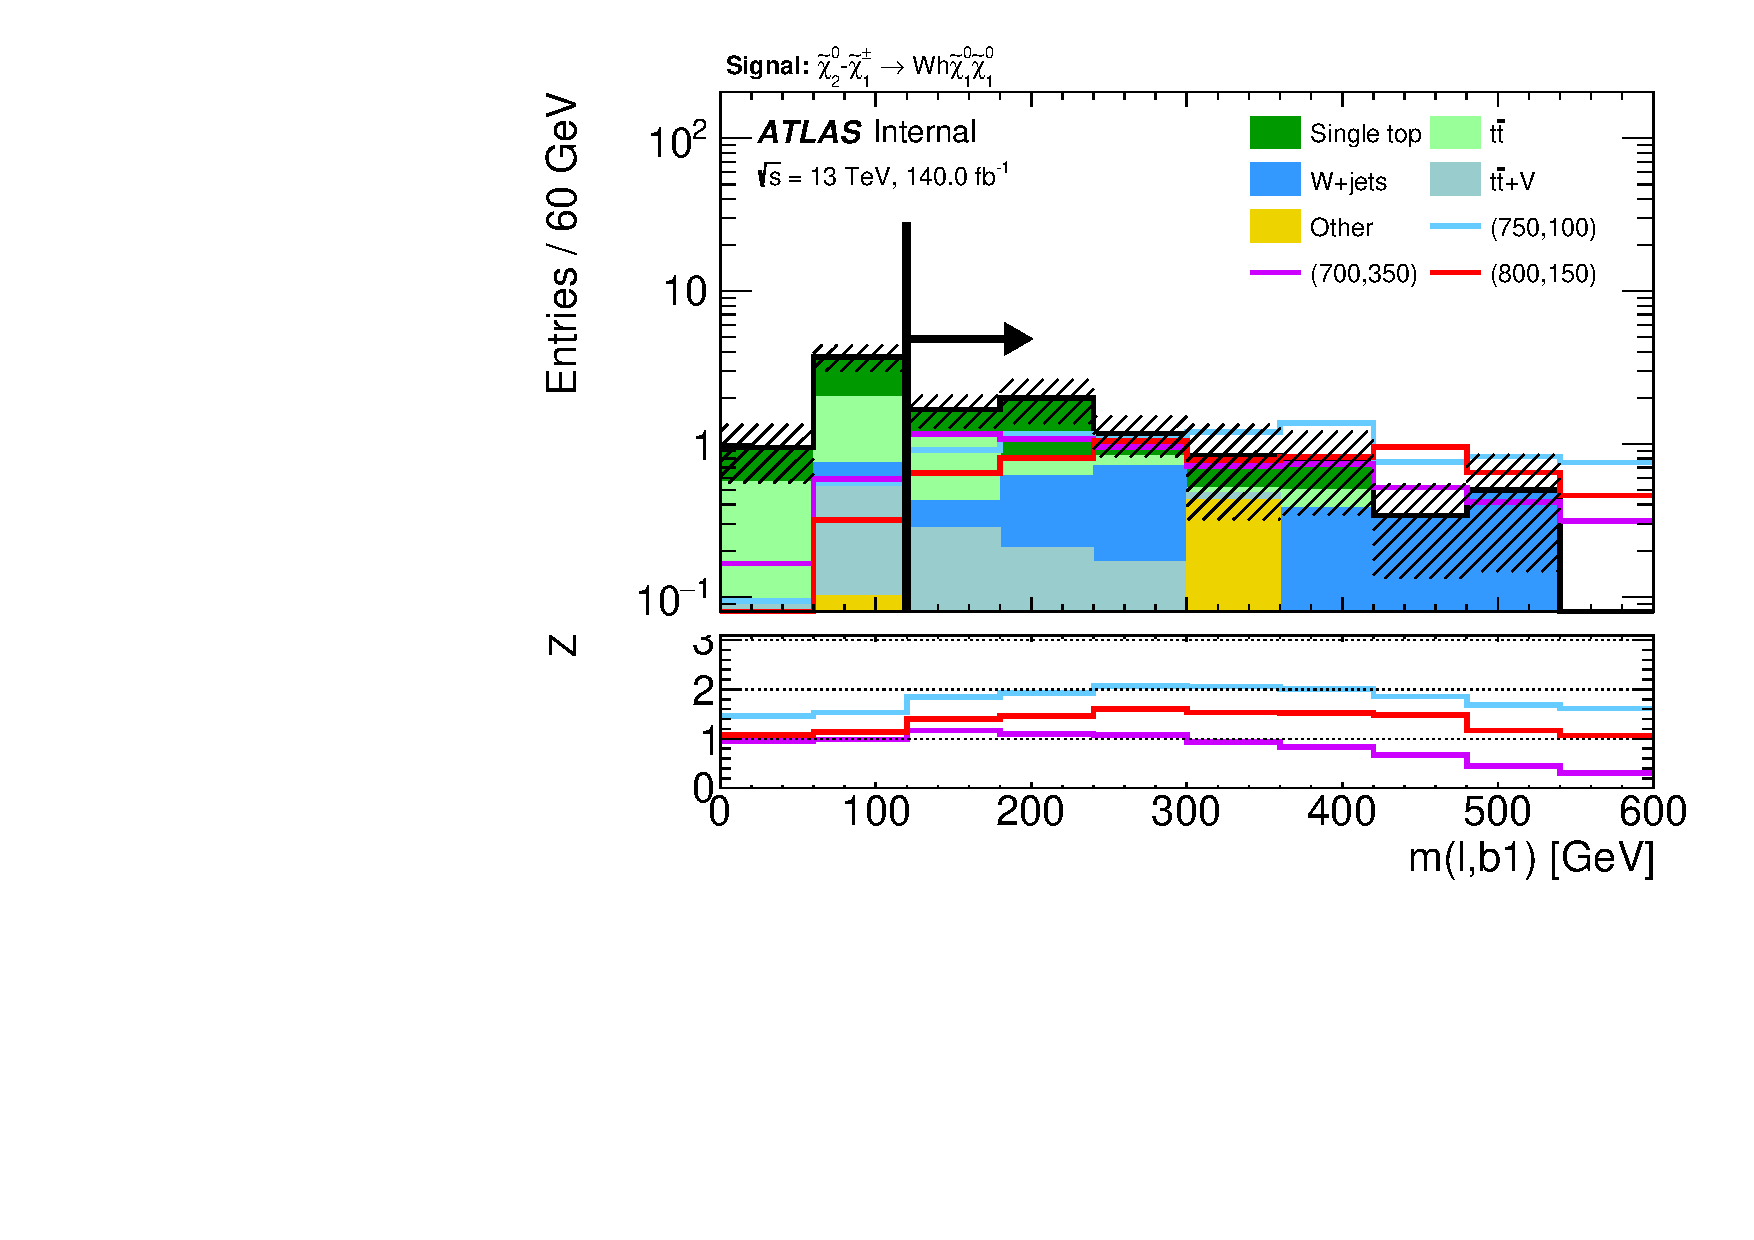
\includegraphics[width=\textwidth]{n1_SRHM_mct_bins/mlb1.pdf}
		\vspace{-2em}
		\caption{\label{fig:Wh_reopt_second_round_n1_srhm_mlb1}}
	\end{subfigure}%
	\begin{subfigure}[b]{0.45\linewidth}
		\centering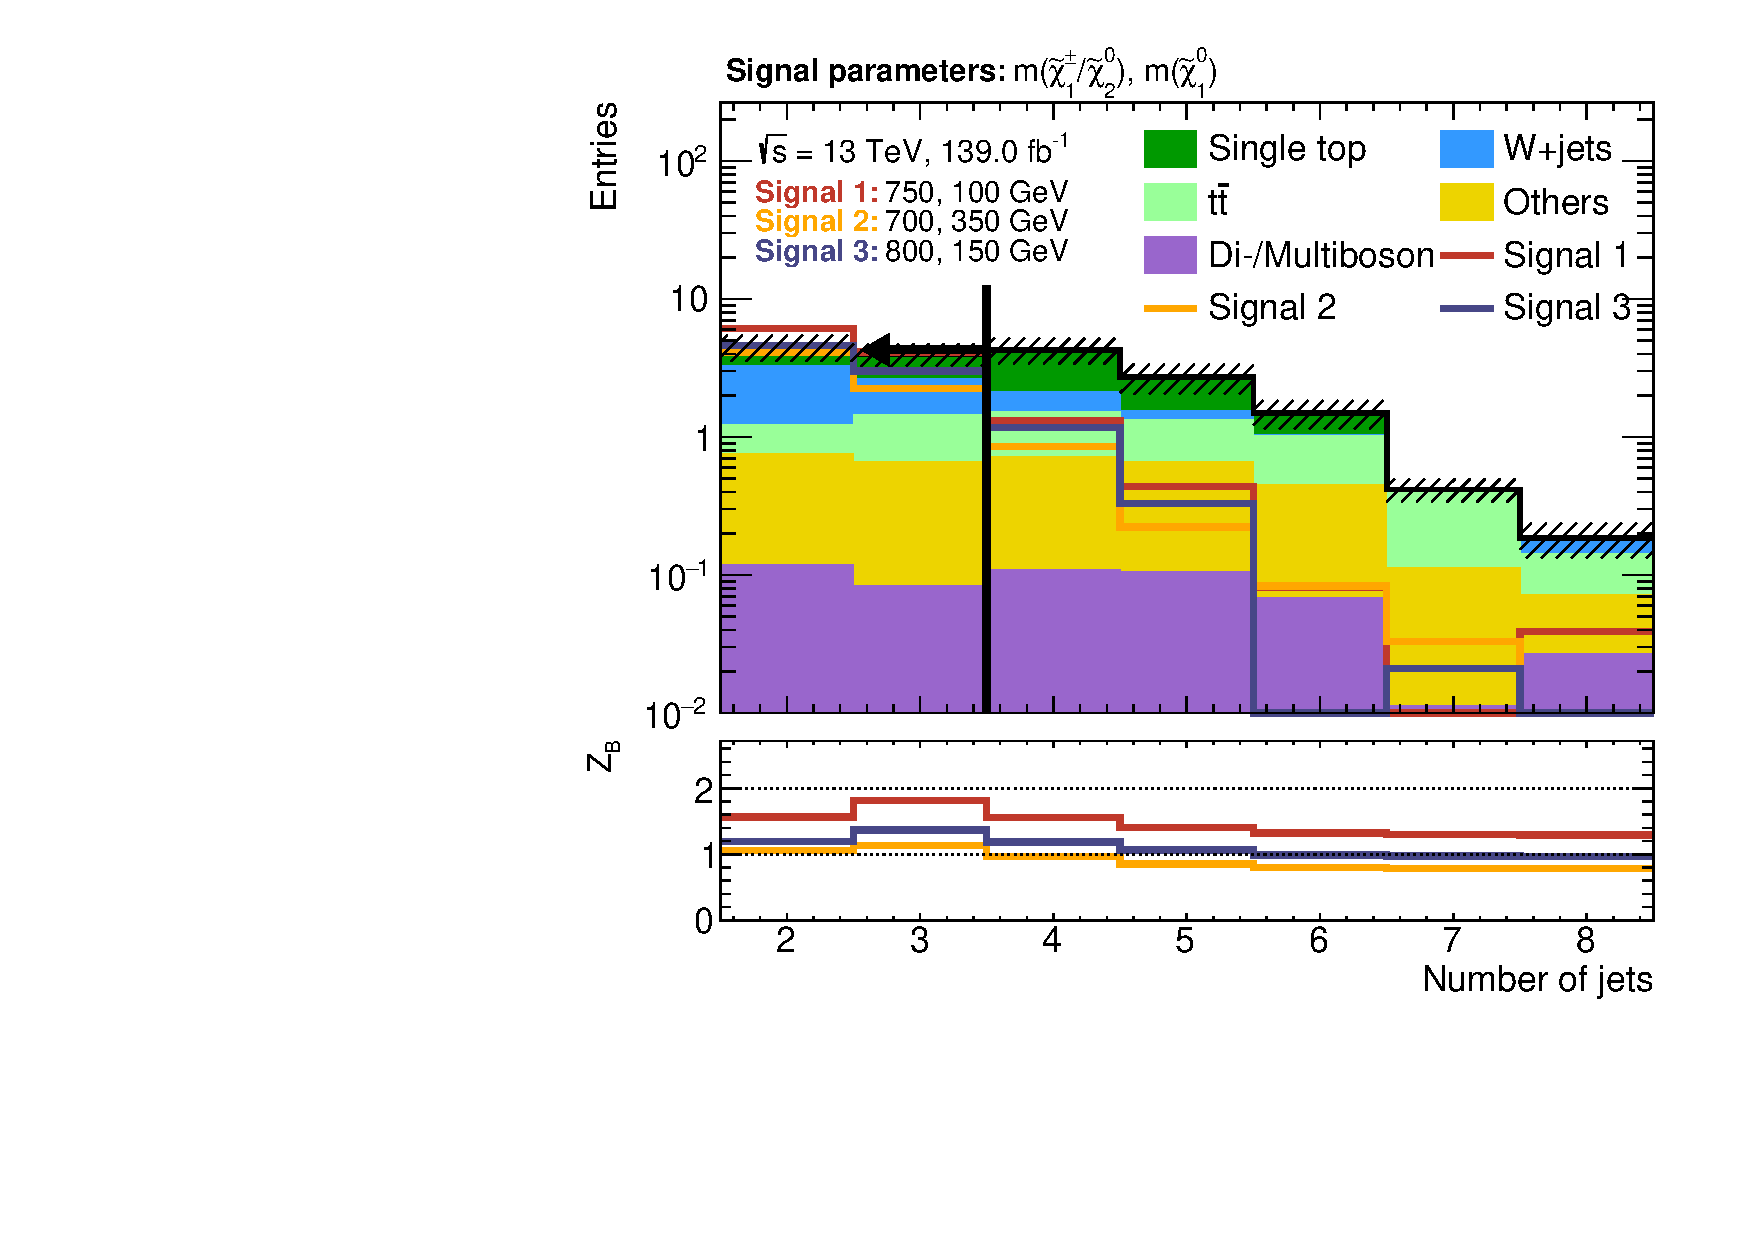
\includegraphics[width=\textwidth]{n1_SRHM_mct_bins/nJet30.pdf}
		\vspace{-2em}
		\caption{\label{fig:Wh_reopt_second_round_n1_srhm_njet}}
	\end{subfigure}
	\caption{\textit{N}--1 plots for SR-HM, with representative signal points and all $\mct$ bins included. The dashed area represents the \gls{mc} statistical uncertainties on the background. In all figures except \figname~\subref{fig:Wh_reopt_second_round_n1_srhm_mct}, the significance in the lower pad is obtained by summing up all the events in the direction of the cut arrow and includes 30\% systematic uncertainties as well as MC statistical uncertainties. In \figname~\subref{fig:Wh_reopt_second_round_n1_srhm_mct} the significance is only computed on a bin-by-bin basis, \ie not summing up all events in the direction of the cut arrow.}
	\label{fig:Wh_reopt_second_round_n1_srhm}
\end{figure}




